\documentclass[14pt]{extreport}\usepackage[]{graphicx}\usepackage[]{xcolor}
% maxwidth is the original width if it is less than linewidth
% otherwise use linewidth (to make sure the graphics do not exceed the margin)
\makeatletter
\def\maxwidth{ %
  \ifdim\Gin@nat@width>\linewidth
    \linewidth
  \else
    \Gin@nat@width
  \fi
}
\makeatother

\definecolor{fgcolor}{rgb}{0, 0, 0}
\newcommand{\hlnum}[1]{\textcolor[rgb]{0.69,0.494,0}{#1}}%
\newcommand{\hlstr}[1]{\textcolor[rgb]{0.749,0.012,0.012}{#1}}%
\newcommand{\hlcom}[1]{\textcolor[rgb]{0.514,0.506,0.514}{\textit{#1}}}%
\newcommand{\hlopt}[1]{\textcolor[rgb]{0,0,0}{#1}}%
\newcommand{\hlstd}[1]{\textcolor[rgb]{0,0,0}{#1}}%
\newcommand{\hlkwa}[1]{\textcolor[rgb]{0,0,0}{\textbf{#1}}}%
\newcommand{\hlkwb}[1]{\textcolor[rgb]{0,0.341,0.682}{#1}}%
\newcommand{\hlkwc}[1]{\textcolor[rgb]{0,0,0}{\textbf{#1}}}%
\newcommand{\hlkwd}[1]{\textcolor[rgb]{0.004,0.004,0.506}{#1}}%
\let\hlipl\hlkwb

\usepackage{framed}
\makeatletter
\newenvironment{kframe}{%
 \def\at@end@of@kframe{}%
 \ifinner\ifhmode%
  \def\at@end@of@kframe{\end{minipage}}%
  \begin{minipage}{\columnwidth}%
 \fi\fi%
 \def\FrameCommand##1{\hskip\@totalleftmargin \hskip-\fboxsep
 \colorbox{shadecolor}{##1}\hskip-\fboxsep
     % There is no \\@totalrightmargin, so:
     \hskip-\linewidth \hskip-\@totalleftmargin \hskip\columnwidth}%
 \MakeFramed {\advance\hsize-\width
   \@totalleftmargin\z@ \linewidth\hsize
   \@setminipage}}%
 {\par\unskip\endMakeFramed%
 \at@end@of@kframe}
\makeatother

\definecolor{shadecolor}{rgb}{.97, .97, .97}
\definecolor{messagecolor}{rgb}{0, 0, 0}
\definecolor{warningcolor}{rgb}{1, 0, 1}
\definecolor{errorcolor}{rgb}{1, 0, 0}
\newenvironment{knitrout}{}{} % an empty environment to be redefined in TeX

\usepackage{alltt}
\setcounter{secnumdepth}{3}
\usepackage[left=3cm,right=3cm,top=2cm,bottom=2cm]{geometry} % page settings
\usepackage{amsmath} 
\usepackage{amsfonts} 
\usepackage[english]{babel} 
\usepackage[round]{natbib}
\usepackage{color}
\usepackage[english]{babel}
\usepackage[utf8]{inputenc}
\setlength{\parindent}{0mm}



%%%%%%%%%%%%%%%%%%%%%%%%%%%%%%%%%%%%%%%%
% This removes the Chapter-Level (Only Sections then!)
\renewcommand{\thesection}{\arabic{section}}

% 
% \usepackage{titlesec}
% \setcounter{secnumdepth}{4}
% 
% \titleformat{\paragraph}
% {\normalfont\normalsize\bfseries}{\theparagraph}{1em}{}
% \titlespacing*{\paragraph}
% {0pt}{3.25ex plus 1ex minus .2ex}{1.5ex plus .2ex}


%%%%%%%%%%%%%%%%%%%%%%%%%%%%%%%%%%%%%%%
% Own Defs:
\newtheorem{theorem}{Theorem}[section]
\newtheorem{lemma}[theorem]{Lemma}
\newtheorem{proposition}[theorem]{Proposition}
\newtheorem{corollary}[theorem]{Corollary}
%%%
\DeclareMathOperator{\trace}{trace}
\DeclareMathOperator{\rank}{rank}
\DeclareMathOperator{\myspan}{span}
\DeclareMathOperator{\Cov}{Cov}
\DeclareMathOperator{\bfbeta}{\boldsymbol{\beta}}
\DeclareMathOperator{\bfW}{\mathbf{W}}
\DeclareMathOperator{\bfSigma}{\boldsymbol{\Sigma}}
\DeclareMathOperator{\bfsigma}{\boldsymbol{\sigma}}
\DeclareMathOperator{\bftheta}{\boldsymbol{\theta}}
\DeclareMathOperator{\bfeps}{\boldsymbol{\varepsilon}}
\DeclareMathOperator{\eps}{\varepsilon}
\DeclareMathOperator{\E}{\mathbb{E}}
\DeclareMathOperator{\V}{\mathbb{V}}
\DeclareMathOperator{\R}{\mathbb{R}}
%\DeclareMathOperator{\P}{\mathbb{P}}
%\DeclareMathOperator{\Cov}{Cov}
\DeclareMathOperator{\AVar}{AVar}
\DeclareMathOperator{\myb}{\mathbf{b}}
\DeclareMathOperator{\X}{\mathbf{X}}
\DeclareMathOperator{\Z}{\mathbf{Z}}
\DeclareMathOperator{\plim}{plim}
\DeclareMathOperator{\toprob}{\overset{p}{\longrightarrow}}
\DeclareMathOperator{\toas}{\overset{a.s.}{\longrightarrow}}
\DeclareMathOperator{\toms}{\overset{m.s.}{\longrightarrow}}
\DeclareMathOperator{\todistr}{\overset{L}{\longrightarrow}}
%%%%%%%%%%%%%%%%%%%%%%%%%%%%%%%%%%%
\newcommand\blfootnote[1]{%
  \begingroup
  \renewcommand\thefootnote{}\footnote{#1}%
  \addtocounter{footnote}{-1}%
  \endgroup
}
%%%%%%%%%%%%%%%%%%%%%%%%%%%%%%%%%%%%%%%
% Fancy Headers and Footers
\usepackage{fancyhdr} 
\pagestyle{fancy}
\fancyhf{}
\renewcommand{\headrulewidth}{0pt} % Remove headings-line
% \rhead{Winter Term 14/15}
% \lhead{Econometrics I (BGSE)}
\rfoot{\thesection-\thepage}
\lfoot{Project Module E\&S}


%%%%%%%%%%%%%%%%%%%%%%%%%%%%%%%%
% Colored Boxes:
\usepackage[framemethod=tikz]{mdframed}
\usepackage[babel=true]{csquotes}
%\definecolor{MidnightBlue}{rgb}{0, 0, 0.551}
%%%%%%%%%%%%%%%%%%%%%%%%%%%%%%%%

\IfFileExists{upquote.sty}{\usepackage{upquote}}{}
\begin{document}
 
% \title{\textbf\Huge Econometrics I (BGSE)}
% \author{Winter Term 2014/15\\Dominik Liebl}
% \date{\today}
% \maketitle


% Knitr Options:


\setcounter{section}{3}
\section{Nonparametric Regression}

Let us consider the case of the case of univariate nonparametric regression, i.e., with one single explanatory variable $X\in\R$.

\bigbreak\noindent {\bf Data:} $(Y_{i},X_{i})$, $i=1,\dots,n$, where
\begin{itemize}
\item $Y_{i}$ response variable
\item $X_{i}\in [a,b]\subset \R$ explanatory  variable
\item $n$ sufficiently large (e.g., $n\geq 40$)
\end{itemize}

\bigskip
\noindent 
\textbf{The Nonparametric Regression Model:}

\smallskip
$$Y_i=m(X_i)+\epsilon_i$$

\begin{itemize}
\item $m(X_i)=\E(Y_i|X=X_i)$ regression function
\item $\epsilon_1,\epsilon_2,\dots$ i.i.d., $\E(\epsilon_i)=0$, $\V(\epsilon_i)=\sigma^2$
\item $\epsilon_i$  independent of $X_i$.
\end{itemize}
\bigbreak
\bigskip

Special cases of \textbf{parametric}  regression models:

\begin{itemize}
\item Linear regression: $m(x)$ is a straight line
$$m(X)=\beta_0+\beta_1 X$$
\item Possible generalizations: $m(x)$ quadratic or cubic
polynomial
\begin{align*}
m(X)&=\beta_0 +\beta_1 X+\beta_2 X^2\\
\text{or} \quad m(X)&=\beta_0+\beta_1 X+\beta_2 X^2+\beta_3 X^3
\end{align*}

\end{itemize}

Many important applications lead to regression functions
possessing a complicated structure. Standard models then are
"too simple" and do not provide useful approximations
of $m(x)$

%\bigskip

\begin{mdframed}[hidealllines=true,backgroundcolor=gray!20]%
 ''All models are {\it false}, but some are useful'' (G. Box)
\end{mdframed}

\newpage

\textbf{Example:}
Canadian cross-section wage data consisting of a random sample taken from the 1971 Canadian Census Public Use Tapes for male individuals having common education (grade 13). 

\begin{knitrout}
\definecolor{shadecolor}{rgb}{0.878, 0.918, 0.933}\color{fgcolor}\begin{kframe}
\begin{alltt}
\hlkwd{library}\hlstd{(}\hlstr{"np"}\hlstd{)}
\hlkwd{data}\hlstd{(}\hlstr{"cps71"}\hlstd{)}
\hlkwd{plot}\hlstd{(cps71}\hlopt{$}\hlstd{age, cps71}\hlopt{$}\hlstd{logwage,} \hlkwc{xlab}\hlstd{=}\hlstr{"Age"}\hlstd{,} \hlkwc{ylab}\hlstd{=}\hlstr{"log(wage)"}\hlstd{)}
\end{alltt}
\end{kframe}

{\centering 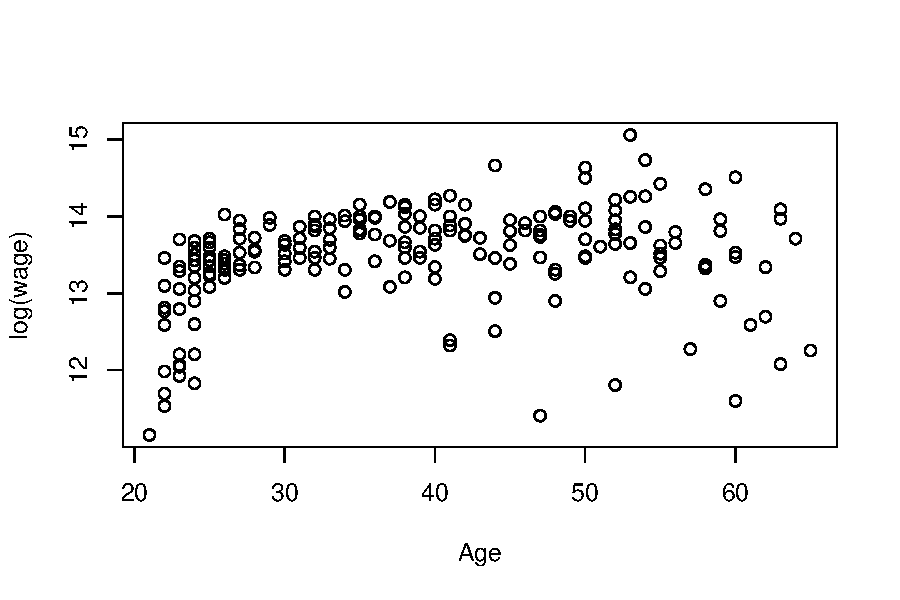
\includegraphics[width=\maxwidth]{figure/unnamed-chunk-1-1} 

}


\end{knitrout}



\textbf{Nonparametric Regression:} 

There are no specific assumptions about the structure
of the regression function. It is only assumed that $m$ is \textit{smooth}.

\bigskip

An important point in theoretical analysis is the way how the observations
 $X_1,\dots,X_n$ have been generated. One distinguishes between ''fixed'' and
''random design''.

\begin{description}
\item[{\bf Fixed design:}]
The observation points $X_1,\dots,X_n$ are fixed  (non stochastic) values.
Example: Crop yield ($Y$) in dependence of the amount of fertilizer ($X$) used.
\item[{\bf Equidistant Design:}]  (most important special case of fixed design)  $$X_{i+1}-X_i=\frac{b-a}{n}.$$
\item[{\bf Random design:}] The observation points $X_1,\dots,X_n$ are (realizations of ) i.i.d. random variables with
density $f$. The density $f$ is called ''design density''. Throughout this chapter it will be assumed that $f(x)>0$ for all
$x\in [a,b]$.

\bigskip
Example: Sample $(Y_1,X_1),\dots,(Y_n,X_n)$ of log-wages ($Y$) and age ($X$) of
randomly selected individuals.\\
In the case of random design $m(x)$ is the conditional expectation of $Y$ given $X=x$,
$$m(x)=\E(Y|\ X=x)$$
and $\V(\epsilon_i|X_i)=\sigma^2$.
Note: For random design all expectations (as well as variances) have to be interpreted as
{\em conditional} expectations (variances) given $X_1,\dots,X_n$.
\end{description}

\subsection{Basis function expansions}

Some frequently used approaches to nonparametric regression rely on expansions of the form
$$
m(x)\approx \sum_{j=1}^p \beta_j b_j(x),
$$
where $b_1(x),b_2(x),\dots$ are suitable basis functions. 

\bigskip

The basis functions $b_1,b_2,\dots$ have to be chosen in such a way that for
{\em any possible} smooth function $m$ the approximation error 
$$
\min_\beta |m(x)-\sum_{j=1}^p \beta_j b_j(x)|$$ 
tends to zero as $p\rightarrow\infty$ (approximation theory).

\bigskip


For a fixed value $p$ an estimator $\hat m_p$ is determined by
$$
\hat m(x)=\sum_{j=1}^p \hat\beta_j b_j(x),
$$
where the coefficients  $\hat\beta_j$ are obtained by ordinary least squares
$$
\sum_{i=1}^n \left( Y_i-\sum_{j=1}^p \hat\beta_j b_j(X_i)\right)^2
=\min_{\beta_1,\dots,\beta_p} \sum_{i=1}^n \left( Y_i-\sum_{j=1}^p \beta_j \underbrace{b_j(X_i)}_{X_{ij}}\right)^2
$$

\bigskip


Examples are approximations by polynomials, spline functions, wavelets or Fourier expansions (for periodic functions).


\subsubsection{Polynomial Regression}

\noindent 
\textbf{Theoretical Justification:} Every smooth function can be well approximated by a polynomial of sufficiently high degree (approximation theory).
\par\noindent

\bigskip

{\bf Approach:}
\begin{itemize}
\item Choose $p$ and fit a polynomial of degree $p$:
$$\min_{\beta_1,\dots,\beta_p}\sum_{i=1}^n \biggl(Y_i-
\sum_{j=1}^p {\beta}_{j} X^{j-1}\biggr)^2$$
$$\Rightarrow\quad {\hat m}_p(X)={\hat \beta}_{1}+\sum_{j=2}^{p-1}
{\hat \beta}_{j} X_i^{j-1}$$
\item This corresponds to an approximation with basis functions
 $$
 b_1(x)=1,b_2(x)=x,b_3(x)=x^2,\dots, b_{p}(x)=x^{p-1}.
 $$
\item  Note: It is only assumed that $m$ is well approximated by a polynomial of degree $p$. That is, there will usually still exist an \textbf{approximation error} (i.e., bias $\neq 0$).
\end{itemize}

\newpage

\textbf{R-Code to compute polynomial regressions:}\\
Generate some data:
\begin{knitrout}
\definecolor{shadecolor}{rgb}{0.878, 0.918, 0.933}\color{fgcolor}\begin{kframe}
\begin{alltt}
\hlkwd{set.seed}\hlstd{(}\hlnum{1}\hlstd{)}
\hlcom{# Generate some data: ####################################}
\hlstd{n}      \hlkwb{<-} \hlnum{100}     \hlcom{# Sample Size}
\hlstd{x_vec}  \hlkwb{<-} \hlstd{(}\hlnum{1}\hlopt{:}\hlstd{n)}\hlopt{/}\hlstd{n} \hlcom{# Equidistant X }
\hlcom{# Gaussian iid error term }
\hlstd{e_vec}  \hlkwb{<-} \hlkwd{rnorm}\hlstd{(}\hlkwc{n} \hlstd{= n,} \hlkwc{mean} \hlstd{=} \hlnum{0}\hlstd{,} \hlkwc{sd} \hlstd{=} \hlnum{.5}\hlstd{)}
\hlcom{# Dependent variable Y}
\hlstd{y_vec}  \hlkwb{<-}  \hlkwd{sin}\hlstd{(x_vec} \hlopt{*} \hlnum{5}\hlstd{)} \hlopt{+} \hlstd{e_vec}
\hlcom{# Save all in a dataframe}
\hlstd{db}     \hlkwb{<-}  \hlkwd{data.frame}\hlstd{(}\hlkwc{x}\hlstd{=x_vec,}\hlkwc{y}\hlstd{=y_vec)}
\hlcom{#########################################################}
\end{alltt}
\end{kframe}
\end{knitrout}
Compute the ordinary least squares regressions of different polynomial regression models:
\begin{knitrout}
\definecolor{shadecolor}{rgb}{0.878, 0.918, 0.933}\color{fgcolor}\begin{kframe}
\begin{alltt}
\hlcom{# Fitting of polynomials to the data (parametric models):}
\hlcom{# Constant line fit: (Basis function x^0)}
\hlstd{reg_1} \hlkwb{<-} \hlkwd{lm}\hlstd{(y} \hlopt{~} \hlnum{1}\hlstd{,} \hlkwc{data}\hlstd{=db)}
\hlcom{# Basis functions: x^0 + ... + x^5}
\hlstd{reg_2} \hlkwb{<-} \hlkwd{lm}\hlstd{(y} \hlopt{~} \hlkwd{poly}\hlstd{(x,} \hlkwc{degree} \hlstd{=} \hlnum{5}\hlstd{),} \hlkwc{data}\hlstd{=db)}
\hlcom{# Basis functions: x^0 + ... + x^25}
\hlstd{reg_3} \hlkwb{=} \hlkwd{lm}\hlstd{(y} \hlopt{~} \hlkwd{poly}\hlstd{(x,} \hlkwc{degree} \hlstd{=} \hlnum{25}\hlstd{),} \hlkwc{data}\hlstd{=db)}
\end{alltt}
\end{kframe}
\end{knitrout}
Take a look at the fits:
\begin{knitrout}
\definecolor{shadecolor}{rgb}{0.878, 0.918, 0.933}\color{fgcolor}\begin{kframe}
\begin{alltt}
\hlkwd{par}\hlstd{(}\hlkwc{mfrow}\hlstd{=}\hlkwd{c}\hlstd{(}\hlnum{2}\hlstd{,}\hlnum{2}\hlstd{),} \hlkwc{mar}\hlstd{=}\hlkwd{c}\hlstd{(}\hlnum{4.1}\hlstd{,}\hlnum{4.1}\hlstd{,}\hlnum{3.1}\hlstd{,}\hlnum{2.1}\hlstd{))}
\hlkwd{plot}\hlstd{(db,} \hlkwc{main}\hlstd{=}\hlstr{"Truth"}\hlstd{)}
\hlkwd{lines}\hlstd{(}\hlkwc{y}\hlstd{=}\hlkwd{sin}\hlstd{(x_vec} \hlopt{*} \hlnum{5}\hlstd{),} \hlkwc{x}\hlstd{=x_vec,} \hlkwc{col}\hlstd{=}\hlstr{"blue"}\hlstd{,} \hlkwc{lwd}\hlstd{=}\hlnum{1.5}\hlstd{)}
\hlcom{##}
\hlkwd{plot}\hlstd{(db,} \hlkwc{main}\hlstd{=}\hlstr{"Degree 0"}\hlstd{)}
\hlkwd{lines}\hlstd{(}\hlkwc{y} \hlstd{=} \hlkwd{predict}\hlstd{(reg_1,} \hlkwc{newdata} \hlstd{= db),}
      \hlkwc{x} \hlstd{= x_vec,} \hlkwc{col}\hlstd{=}\hlstr{"red"}\hlstd{,} \hlkwc{lwd}\hlstd{=}\hlnum{1.5}\hlstd{)}
\hlkwd{plot}\hlstd{(db,} \hlkwc{main}\hlstd{=}\hlstr{"Degree 5"}\hlstd{)}
\hlkwd{lines}\hlstd{(}\hlkwc{y} \hlstd{=} \hlkwd{predict}\hlstd{(reg_2,} \hlkwc{newdata} \hlstd{= db),}
      \hlkwc{x} \hlstd{= x_vec,} \hlkwc{col}\hlstd{=}\hlstr{"red"}\hlstd{,} \hlkwc{lwd}\hlstd{=}\hlnum{1.5}\hlstd{)}
\hlkwd{plot}\hlstd{(db,} \hlkwc{main}\hlstd{=}\hlstr{"Degree 25"}\hlstd{)}
\hlkwd{lines}\hlstd{(}\hlkwc{y} \hlstd{=} \hlkwd{predict}\hlstd{(reg_3,} \hlkwc{newdata} \hlstd{= db),}
      \hlkwc{x} \hlstd{= x_vec,} \hlkwc{col}\hlstd{=}\hlstr{"red"}\hlstd{,} \hlkwc{lwd}\hlstd{=}\hlnum{1.5}\hlstd{)}
\end{alltt}
\end{kframe}

{\centering 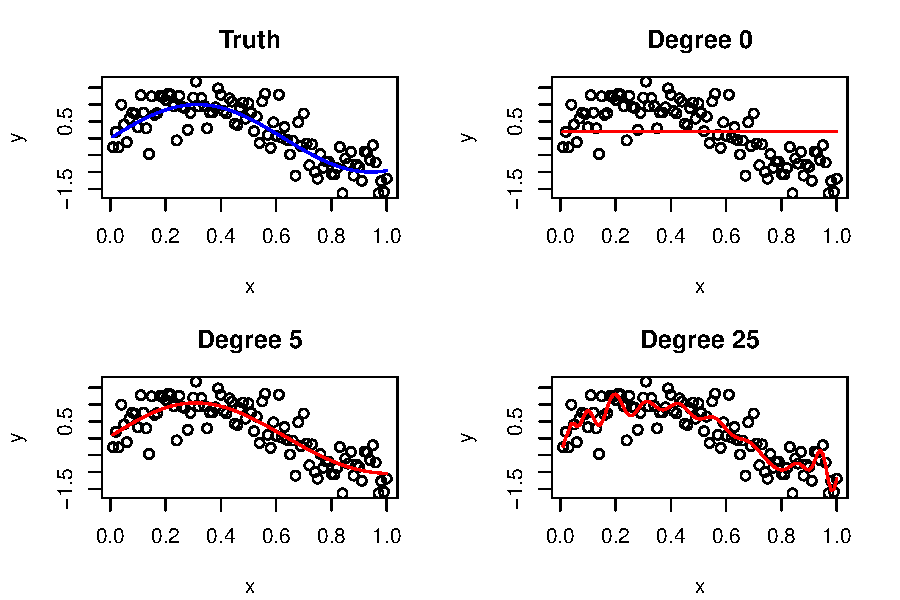
\includegraphics[width=\maxwidth]{figure/unnamed-chunk-4-1} 

}


\end{knitrout}


The quality of the approximation obviously depends on the choice of $p$ which serves as a ''smoothing parameter''


\begin{itemize}
\item $p$ small: variability of the estimator is small, but there may exist a high systematic error (bias).
\item $p$ large: bias is small, but variability of the estimator is high.
\end{itemize}


Remark:\\
Polynomial regression is not very popular in practice. Reasons are numerical problems in fitting high dimensional
polynomials. Furthermore, high order polynomials often posses
an erratic, difficult to interpret behavior at the boundaries.

\newpage

\subsubsection{Regression Splines}

The practical disadvantages of global basis functions (like polynomials), explain the success of local basis functions. A frequently used system of basis functions are {\bf local polynomials}, i.e., so-called ''spline functions''.  

\bigskip


A spline function is a {\em piece wise } polynomial function. They are defined with respect
to a pre-specified sequence of $q$ ''knots'' 
$$
a= \tau_1<\tau_2<\dots<\tau_q= b.
$$ 
Different specifications of the knot sequence lead to different splines.

\bigskip

More precisely, for a given knot sequence a spline function $s(x)$ of degree $k$ is defined by the following properties:
\begin{itemize}
\item $s(x)$ is a polynomial of degree $k$ in every interval $[\tau_j,\tau_{j+1}]$, i.e.
$s(x)=s_0+s_1x+s_2x^2+\dots+s_kx^{k}$, $s_0,\dots,s_k\in\R$, for all $x\in[\tau_j,\tau_{j+1}]$.
\item $s(x)$ is  $k-1$ times continuously differentiable at each knot point $x=\tau_j$, $j=1,\dots,q$.
\end{itemize}

$s(x)$ is called a \emph{linear spline} if $k=1$, $s(x)$ is a \emph{quadratic spline} if $k=2$, and
$s(x)$ is a \emph{cubic spline}  if $k=3$.

\bigskip

In practice, the most frequently used splines are \emph{cubic} spline functions based on an equidistant sequence of $q$ knots, i.e.,
$\tau_{j+1}-\tau_j=\tau_j-\tau_{j-1}\quad\text{for all } j$.

\bigskip

The space of all spline functions of degree $k$ defined with respect to a given knot sequence
$a=\tau_1,\dots,\tau_q\le b$ is a $p:=q+k-1$ dimensional linear function space
${\cal{S}}_{k,\tau_1,\dots,\tau_q}=\operatorname{span}(b_{1,k},\dots,b_{p,k})$.

% \bigskip
% 
% Possible basis functions are\\
% $\tilde{b}_1(x)=1,\tilde{b}_2(x)=x,\dots,\tilde{b}_{k}=x^{k-1},\tilde{b}_{k+1}=(x-\tau_1)^k_+,\dots,
% \tilde{b}_{k+q-1}=(x-\tau_{q-1})^k_+$, where
% $$(x-\tau_j)^k_+=\left\{ \begin{matrix}  (x-\tau_j)^k & \text{ if } x\ge  \tau_j\\
% 0 & \text{ else} \end{matrix}\right.$$
% Each spline function $s\in {\cal{S}}_{k,\tau_1,\dots,\tau_q}$ can then be written as
% 
% $$s(x)=\sum_{j=1}^{k} \beta_{j} x^{j-1} +\sum_{j=1}^{q-1}\beta_{j+k}(x-\tau_j)^k_+\quad\text{ for } x\in[a,b]$$
% and suitable parameters $\beta_1,\dots,\beta_{k+q-2}$.

\bigskip

\textbf{B-Spline Basis Functions:} The so-called B-spline basis functions are almost always used in practice, since they possess a number of advantages from a numerical point of view.

\bigskip

The B-Spline basis functions $b_{j,k}$, $j=1,\dots,k+q-2$, for splines of order $k$ based on a knot sequence $a\le \tau_1,\dots,\tau_q\le b$
  are calculated by a recursive procedure:
$$b_{j,0}(x)=\left\{ \begin{matrix}  1 & \text{ if } x\in[\tau_{j}^*,\tau_{j+1}^*]\\
0 & \text{ else} \end{matrix}\right., \quad j=1,\dots,q+2k-1 $$
and
$$b_{j,l}(x)=\frac{x-\tau_j^*}{\tau_{l+j}^*-\tau_j^*}b_{j,l-1}(x)+
\frac{\tau_{l+j+1}^*-x}{\tau_{l+j+1}^*-\tau_{j+1}^*}b_{j+1,l-1}(x),
$$
for $l=1,\dots,k$, $j=1,\dots,q+k-1$, and $x\in [a,b]$. Here, $\tau_1^*=\dots=\tau_{k+1}^*=\tau_1$,
$\tau_{k+2}^*=\tau_2,\dots,\tau^*_{k+q}=\tau_q$ and $\tau_{k+q+1}^*=\dots=\tau_{2k+q}^*=\tau_q$.

\bigskip

\textbf{R-Code to generate B-Spline basis functions:}\\
Generate cubic ($k=3$) B-spline functions for an equidistant knot sequence
with $\tau_1=0,\,\tau_2=0.25,\,\tau_3=0.5,\,\tau_4=0.75,\,\tau_5=1$.
\begin{knitrout}
\definecolor{shadecolor}{rgb}{0.878, 0.918, 0.933}\color{fgcolor}\begin{kframe}
\begin{alltt}
\hlkwd{suppressMessages}\hlstd{(}\hlkwd{library}\hlstd{(}\hlstr{"fda"}\hlstd{))}
\hlstd{degree}   \hlkwb{<-} \hlnum{3} \hlcom{# piecewise cubic splines}
\hlstd{knot.seq} \hlkwb{<-} \hlkwd{seq}\hlstd{(}\hlkwc{from}\hlstd{=}\hlnum{0}\hlstd{,}\hlkwc{to}\hlstd{=}\hlnum{1}\hlstd{,}\hlkwc{len}\hlstd{=}\hlnum{5}\hlstd{)}\hlcom{# knots}
\hlstd{knot.seq}
\end{alltt}
\begin{verbatim}
## [1] 0.00 0.25 0.50 0.75 1.00
\end{verbatim}
\begin{alltt}
\hlstd{cubic.spl} \hlkwb{<-} \hlkwd{create.bspline.basis}\hlstd{(}
             \hlkwc{norder} \hlstd{= degree} \hlopt{+} \hlnum{1}\hlstd{,} \hlcom{# order=degree+1  }
             \hlkwc{breaks} \hlstd{= knot.seq)}
\end{alltt}
\end{kframe}
\end{knitrout}

This leads to 
$$
p=\underbrace{\texttt{Numbr.of Knots}}_{q=5} + \underbrace{\texttt{degree}}_{k=3} - 1=7
$$ 
cubic B-spline basis functions. Let's take a look at them:
% which together span the $p=7$ dimensional linear function space $\mathcal{S}_{k=3,\tau_1=0,\dots,\tau_5=1}=\operatorname{span}(b_{1,k=3},\dots,b_{7,k=3})$. 
%\bigskip

\begin{knitrout}
\definecolor{shadecolor}{rgb}{0.878, 0.918, 0.933}\color{fgcolor}\begin{kframe}
\begin{alltt}
\hlcom{# evaluation grid}
\hlstd{eval_grid}     \hlkwb{<-} \hlkwd{seq}\hlstd{(}\hlkwc{from}\hlstd{=}\hlnum{0}\hlstd{,}\hlkwc{to}\hlstd{=}\hlnum{1}\hlstd{,}\hlkwc{len}\hlstd{=}\hlnum{50}\hlstd{)}
\hlcom{# evaluate the 7 basis functions at eval_grid:}
\hlstd{X.basis.mat} \hlkwb{<-} \hlkwd{eval.basis}\hlstd{(}\hlkwc{basisobj} \hlstd{= cubic.spl,}
                          \hlkwc{evalarg}  \hlstd{= eval_grid)}
\hlkwd{dim}\hlstd{(X.basis.mat)}
\end{alltt}
\begin{verbatim}
## [1] 50  7
\end{verbatim}
\begin{alltt}
\hlcom{# plot:}
\hlkwd{matplot}\hlstd{(}\hlkwc{y}\hlstd{=X.basis.mat,} \hlkwc{x}\hlstd{=eval_grid,} \hlkwc{type}\hlstd{=}\hlstr{"l"}\hlstd{,} \hlkwc{lwd}\hlstd{=}\hlnum{1.5}\hlstd{,}
        \hlkwc{axes}\hlstd{=F,} \hlkwc{ylab}\hlstd{=}\hlstr{""}\hlstd{,} \hlkwc{xlab}\hlstd{=}\hlstr{"Knots"}\hlstd{,}
        \hlkwc{main}\hlstd{=}\hlstr{"Cubic B-Spline Basis Functions"}\hlstd{)}
\hlkwd{axis}\hlstd{(}\hlnum{1}\hlstd{,} \hlkwc{at}\hlstd{=knot.seq);} \hlkwd{axis}\hlstd{(}\hlnum{2}\hlstd{);} \hlkwd{box}\hlstd{()}
\end{alltt}
\end{kframe}

{\centering 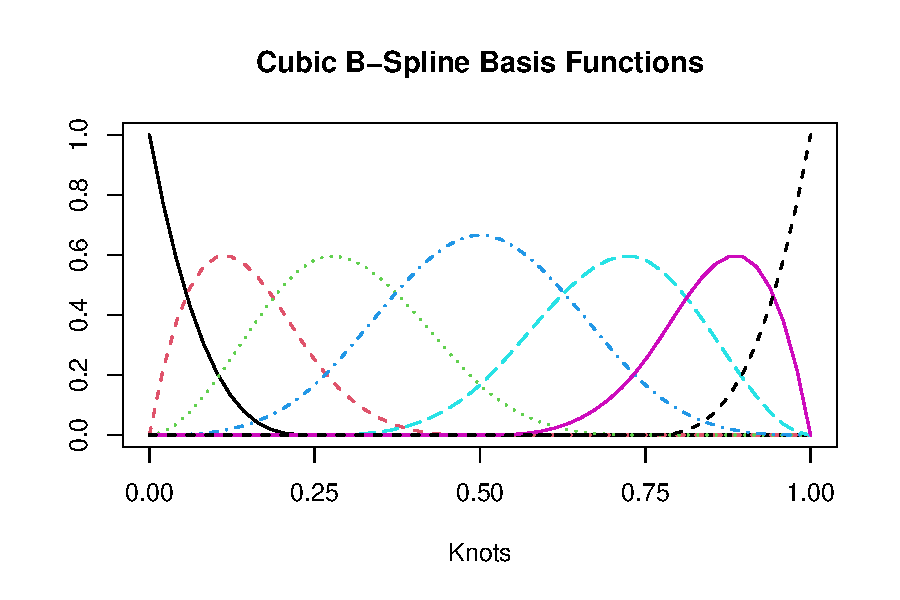
\includegraphics[width=\maxwidth]{figure/unnamed-chunk-6-1} 

}


\end{knitrout}


\textbf{Regression Splines:}

\bigskip

The so-called ''regression spline'' (or ''B-spline'') approach to estimating a regression function $m(x)$ is based
on fitting a set of spline basis functions to the data. Frequently, cubic splines ($k=3$) with equidistant knots are applied. Then $\tau_1=a, \tau_q=b$ and
$\tau_{j+1}-\tau_j=(b-a)/(q-1)$. 

\bigskip

In this case the number of knots $q$ (or more precisely the total number of basis functions $p=q+k-1$ with $k=3$ in the case of cubic B-splines) serves as the ''\textbf{smoothing parameter}''
which has to be selected by the statistician.

\bigskip

An estimator $\hat m_p(x)$ is then given by
$$\hat m_p(x)=\sum_{j=1}^p \hat\beta_j b_{j,k}(x),$$
 and the coefficients $\hat\beta_j$ are determined by ordinary
least squares.

\bigskip

Let $Y=(Y_1,\dots,Y_n)^\top $ denote the vector of response variables and let $\mathbf{X}$ denote the $n\times p$ matrix with elements $X_{ij}=b_{j,k}(X_i)$.

\bigskip

Then the OLS estimate 
$\hat \beta=(\hat\beta_1,\dots,\hat\beta_p)^\top $ can be written as
$$
\hat\beta=(\mathbf{X}^\top \mathbf{X})^{-1}\mathbf{X}^\top Y.
$$
The fitted values are given by
$$
% \left(\begin{array}{c}
% {\hat Y}_1\\
% \vdots%\\ \cdot\\ \cdot
% \\ {\hat Y}_n
% \end{array}\right)=
\left(\begin{array}{c}
{\hat m}_p(X_1)\\
\vdots%\\ \cdot\\ \cdot
\\ {\hat m}_p(X_n)
\end{array}\right)=\mathbf{X}\hat\beta=\underbrace{\mathbf{X}(\mathbf{X}^\top \mathbf{X})^{-1}\mathbf{X}^\top }_{=:S_p}Y
$$

The matrix $S_p$ is referred to as the \textbf{smoothing matrix} and the number of B-spline basis function $p$ is referred to as the \textbf{smoothing parameter}. 

\bigskip

Remark: Quite generally, the most important nonparametric regression procedures are ``linear smoothing methods''. This means that in dependence of some smoothing parameter (here $p$), estimates of the vector
$(m(X_1),\dots,m(X_n))^\top $ are obtained by multiplying a ``smoother matrix'' $S_p$ with $Y$. That is, 

$$
\left(\begin{array}{c}
m(X_1)\\
\vdots%\\ \cdot\\ \cdot
\\ m(X_n)
\end{array}\right)\approx
\left(\begin{array}{c}
{\hat m}_p(X_1)\\
\vdots%\\ \cdot\\ \cdot
\\ {\hat m}_p(X_n)
\end{array}\right)=S_p Y
$$


\newpage

\textbf{R-Code to compute regression splines:}\\
Generate some data:
\begin{knitrout}
\definecolor{shadecolor}{rgb}{0.878, 0.918, 0.933}\color{fgcolor}\begin{kframe}
\begin{alltt}
\hlkwd{set.seed}\hlstd{(}\hlnum{1}\hlstd{)}
\hlcom{# Generate some data: ####################################}
\hlstd{n}      \hlkwb{<-} \hlnum{100}     \hlcom{# Sample Size}
\hlstd{x_vec}  \hlkwb{<-} \hlstd{(}\hlnum{1}\hlopt{:}\hlstd{n)}\hlopt{/}\hlstd{n} \hlcom{# Equidistant X }
\hlcom{# Gaussian iid error term }
\hlstd{e_vec}  \hlkwb{<-} \hlkwd{rnorm}\hlstd{(}\hlkwc{n} \hlstd{= n,} \hlkwc{mean} \hlstd{=} \hlnum{0}\hlstd{,} \hlkwc{sd} \hlstd{=} \hlnum{.5}\hlstd{)}
\hlcom{# Dependent variable Y}
\hlstd{y_vec}  \hlkwb{<-}  \hlkwd{sin}\hlstd{(x_vec} \hlopt{*} \hlnum{5}\hlstd{)} \hlopt{+} \hlstd{e_vec}
\hlcom{#########################################################}
\end{alltt}
\end{kframe}
\end{knitrout}
Generate cubic B-spline basis functions with equidistant knot sequence \texttt{seq(from=0,to=1,len=15)} and evaluate them at \texttt{x\_vec}:%0.01, 0.02, 0.03, 0.04, 0.05, 0.06, 0.07, 0.08, 0.09, 0.1, 0.11, 0.12, 0.13, 0.14, 0.15, 0.16, 0.17, 0.18, 0.19, 0.2, 0.21, 0.22, 0.23, 0.24, 0.25, 0.26, 0.27, 0.28, 0.29, 0.3, 0.31, 0.32, 0.33, 0.34, 0.35, 0.36, 0.37, 0.38, 0.39, 0.4, 0.41, 0.42, 0.43, 0.44, 0.45, 0.46, 0.47, 0.48, 0.49, 0.5, 0.51, 0.52, 0.53, 0.54, 0.55, 0.56, 0.57, 0.58, 0.59, 0.6, 0.61, 0.62, 0.63, 0.64, 0.65, 0.66, 0.67, 0.68, 0.69, 0.7, 0.71, 0.72, 0.73, 0.74, 0.75, 0.76, 0.77, 0.78, 0.79, 0.8, 0.81, 0.82, 0.83, 0.84, 0.85, 0.86, 0.87, 0.88, 0.89, 0.9, 0.91, 0.92, 0.93, 0.94, 0.95, 0.96, 0.97, 0.98, 0.99, 1: 
\begin{knitrout}
\definecolor{shadecolor}{rgb}{0.878, 0.918, 0.933}\color{fgcolor}\begin{kframe}
\begin{alltt}
\hlstd{degree}      \hlkwb{<-} \hlnum{3} \hlcom{# piecewise cubic splines}
\hlstd{knot.seq.5}  \hlkwb{<-} \hlkwd{seq}\hlstd{(}\hlkwc{from}\hlstd{=}\hlnum{0}\hlstd{,}\hlkwc{to}\hlstd{=}\hlnum{1}\hlstd{,}\hlkwc{len}\hlstd{=}\hlnum{5}\hlstd{)}\hlcom{# knots}
\hlstd{cubic.spl.7} \hlkwb{<-} \hlkwd{create.bspline.basis}\hlstd{(}
                \hlkwc{norder} \hlstd{= degree} \hlopt{+} \hlnum{1}\hlstd{,} \hlcom{# order=degree+1}
                \hlkwc{breaks} \hlstd{= knot.seq.5)}
\hlstd{knot.seq.15}  \hlkwb{<-} \hlkwd{seq}\hlstd{(}\hlkwc{from}\hlstd{=}\hlnum{0}\hlstd{,}\hlkwc{to}\hlstd{=}\hlnum{1}\hlstd{,}\hlkwc{len}\hlstd{=}\hlnum{15}\hlstd{)}\hlcom{# knots}
\hlstd{cubic.spl.17} \hlkwb{<-} \hlkwd{create.bspline.basis}\hlstd{(}
                \hlkwc{norder} \hlstd{= degree} \hlopt{+} \hlnum{1}\hlstd{,} \hlcom{# order=degree+1}
                \hlkwc{breaks} \hlstd{= knot.seq.15)}

\hlcom{# evaluate the B-spline basis functions at x_vec:}
\hlstd{X.p7}  \hlkwb{<-} \hlkwd{eval.basis}\hlstd{(}\hlkwc{basisobj}\hlstd{=cubic.spl.7,}  \hlkwc{evalarg}\hlstd{=x_vec)}
\hlstd{X.p17} \hlkwb{<-} \hlkwd{eval.basis}\hlstd{(}\hlkwc{basisobj}\hlstd{=cubic.spl.17,} \hlkwc{evalarg}\hlstd{=x_vec)}
\end{alltt}
\end{kframe}
\end{knitrout}
Compute the smoothing matrices $S_p$ for $p=7$ and $p=17$:
\begin{knitrout}
\definecolor{shadecolor}{rgb}{0.878, 0.918, 0.933}\color{fgcolor}\begin{kframe}
\begin{alltt}
\hlstd{S.p7}  \hlkwb{<-} \hlstd{X.p7}  \hlopt \hlkwd{solve}\hlstd{(}\hlkwd{t}\hlstd{(X.p7)}  \hlopt \hlstd{X.p7)}  \hlopt \hlkwd{t}\hlstd{(X.p7)}
\hlstd{S.p17} \hlkwb{<-} \hlstd{X.p17} \hlopt \hlkwd{solve}\hlstd{(}\hlkwd{t}\hlstd{(X.p17)} \hlopt \hlstd{X.p17)} \hlopt \hlkwd{t}\hlstd{(X.p17)}
\end{alltt}
\end{kframe}
\end{knitrout}
Compute the estimates $\hat{m}_p(X_1),\dots,\hat{m}_p(X_n)$ for $p=7$ and $p=17$:
\begin{knitrout}
\definecolor{shadecolor}{rgb}{0.878, 0.918, 0.933}\color{fgcolor}\begin{kframe}
\begin{alltt}
\hlstd{m.hat.p7}  \hlkwb{<-} \hlstd{S.p7}  \hlopt \hlstd{y_vec}
\hlstd{m.hat.p17} \hlkwb{<-} \hlstd{S.p17} \hlopt \hlstd{y_vec}
\end{alltt}
\end{kframe}
\end{knitrout}
Let's plot the results:
\begin{knitrout}
\definecolor{shadecolor}{rgb}{0.878, 0.918, 0.933}\color{fgcolor}\begin{kframe}
\begin{alltt}
\hlkwd{plot}\hlstd{(}\hlkwc{y}\hlstd{=y_vec,} \hlkwc{x}\hlstd{=x_vec,} \hlkwc{xlab}\hlstd{=}\hlstr{"X"}\hlstd{,} \hlkwc{ylab}\hlstd{=}\hlstr{"Y"}\hlstd{,}
     \hlkwc{main}\hlstd{=}\hlstr{"Regression Splines"}\hlstd{)}
\hlkwd{lines}\hlstd{(}\hlkwc{y}\hlstd{=}\hlkwd{sin}\hlstd{(x_vec} \hlopt{*} \hlnum{5}\hlstd{),} \hlkwc{x}\hlstd{=x_vec,} \hlkwc{col}\hlstd{=}\hlstr{"red"}\hlstd{,} \hlkwc{lty}\hlstd{=}\hlnum{2}\hlstd{,} \hlkwc{lwd}\hlstd{=}\hlnum{1.5}\hlstd{)}
\hlkwd{lines}\hlstd{(}\hlkwc{y}\hlstd{=m.hat.p7,} \hlkwc{x}\hlstd{=x_vec,} \hlkwc{col}\hlstd{=}\hlstr{"blue"}\hlstd{,} \hlkwc{lwd}\hlstd{=}\hlnum{1.5}\hlstd{)}
\hlkwd{lines}\hlstd{(}\hlkwc{y}\hlstd{=m.hat.p17,} \hlkwc{x}\hlstd{=x_vec,} \hlkwc{col}\hlstd{=}\hlstr{"darkorange"}\hlstd{,} \hlkwc{lwd}\hlstd{=}\hlnum{1.5}\hlstd{)}
\hlkwd{legend}\hlstd{(}\hlstr{"bottomleft"}\hlstd{,}
       \hlkwd{c}\hlstd{(}\hlstr{"(Unknown) Regression Function m"}\hlstd{,}
         \hlstr{"Regr.-Spline Fit with p=7"}\hlstd{,}
         \hlstr{"Regr.-Spline Fit with p=17"}\hlstd{),}
       \hlkwc{col}\hlstd{=}\hlkwd{c}\hlstd{(}\hlstr{"red"}\hlstd{,}\hlstr{"blue"}\hlstd{,} \hlstr{"darkorange"}\hlstd{),}
       \hlkwc{lty}\hlstd{=}\hlkwd{c}\hlstd{(}\hlnum{2}\hlstd{,}\hlnum{1}\hlstd{,}\hlnum{1}\hlstd{),} \hlkwc{lwd}\hlstd{=}\hlkwd{c}\hlstd{(}\hlnum{2}\hlstd{,}\hlnum{2}\hlstd{,}\hlnum{2}\hlstd{))}
\end{alltt}
\end{kframe}

{\centering 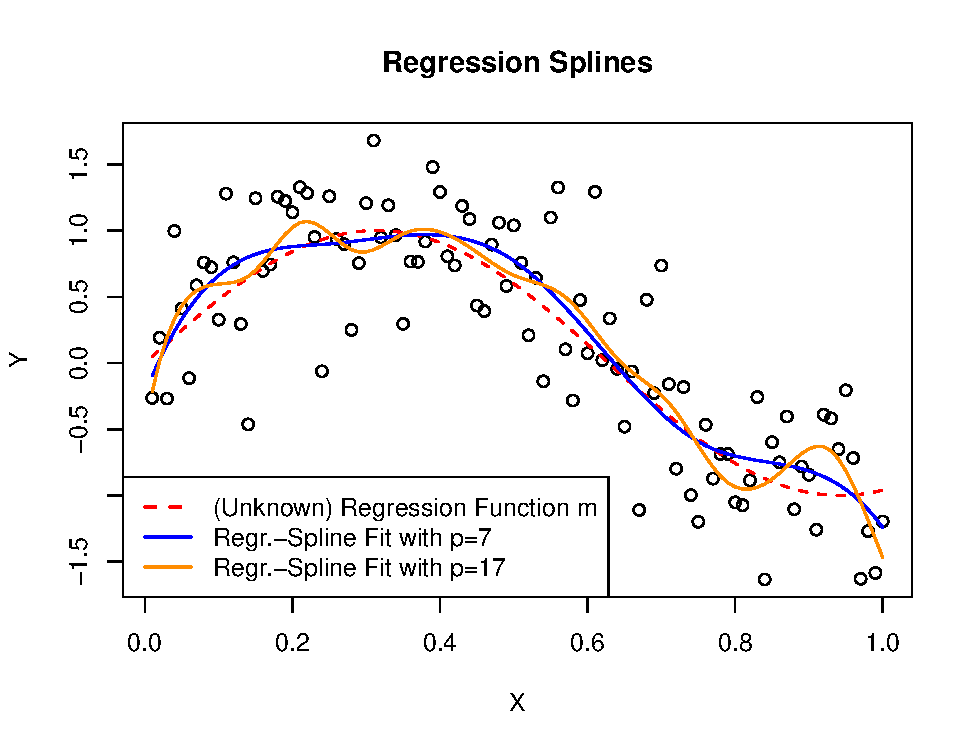
\includegraphics[width=\maxwidth]{figure/unnamed-chunk-11-1} 

}


\end{knitrout}


% \subsubsection{Approximation properties of spline functions}
% 
% As already mentioned above,  nonparametric regression does {\bf not} assume that $m(x)$ exactly corresponds
% to a spline function. $\hat m_p$ thus possesses a systematic error. But if the number of knots is large,
% then splines can {\bf approximate} any smooth function with high accuracy.
% 
% 
% {\bf The accuracy of  spline approximations:} Results of approximation theory imply that  for any
% spline order $k$ and any $\nu-times$ continuously differentiable function $m$, $1\leq \nu\leq k+1$,  we have
% \begin{align*}
% \min_{s\in {\cal{S}}_{k,\tau_1,\dots,\tau_q}}&
% \max_{x\in[a,b]} \left|m(x)-s(x)\right| \\
% &\leq C_{\nu,k}  \max_{j=1,\dots,q}|\tau_{j+1}-\tau_j|^{\nu}
% \max_{x\in[a,b]} |m^{(\nu)}(x)|
% \end{align*}
% for some universal constant $C_{\nu,k}$ which only depends on $\nu$ and $k$.
% 
% \bigbreak
% Let $k=3$ (cubic spline function). A cubic spline function satisfying the boundary constraints
% $s''(\tau_1)=s''(\tau_q)=0$ is usually called a (cubic)
%  ``natural spline''. Note that for any cubic natural spline the effective number of parameters to be
%  estimated reduces to $q$ (instead of $q+2$).
% 
%  Now assume that for some twice continuously differentiable function $m$ only the functional values
%  $m(\tau_1),\dots,m(\tau_q)$ at $\tau_1,\dots,\tau_q$ are known. We then have to {\bf interpolate} these
%  functional values in order to obtain some suitable reconstruction of $m(x)$ on $[\tau_1,\tau_q]$.
% 
%  {\bf Spline interpolation:} For all possible values $m(\tau_1),\dots,m(\tau_q)$ there exists a
%  unique cubic natural spline $s_{m,q}$ interpolating these values, i.e.,   $s_{m,q}(\tau_j)=m(\tau_j)$ for
%  all $j=1,\dots,q$. Spline theory now states that  $s_{m,q}$ is the {\bf smoothest} function interpolating
% these values,
% $$
% \int_{\tau_1}^{\tau_q} s_{m,q}''(x)^2 dx \leq \int_{\tau_1}^{\tau_q} \tilde m''(x)^2 dx$$
% for any other twice cont. differentiable function $\tilde m$ with $\tilde m(\tau_j)=m(\tau_j)$ for
%  all $j=1,\dots,q$.
% 
% {\bf Literature:} C. de Boor,   ''A practical guide to splines'' , Springer  (1978);
% R. Eubank, ''Spline smoothing and nonparametric regression'', Marcel Dekker (1988)
% 

\newpage

\subsubsection{Mean Average Squared Error of Regression Splines}

In a nonparametric regression context we do {\bf not} assume that the unknown true regression function $m(x)$ exactly corresponds
to a spline function. Thus, $\hat m_p=(\hat{m}_p(X_1),\dots,\hat{m}_p(X_n))^\top$ possesses a systematic estimation error (bias). That is, 
$$
\E_\epsilon(\hat m_p(X_i))\neq m(X_i).
$$

To simplify notation, we will in the following write ``$\E_\epsilon$'' as well as ``$\V_\epsilon$'' to denote expectation and variance ``with respect to the random variable $\epsilon$, only''. 

\bigskip

In the case of random design,
``$\E_\epsilon$'' and ``$\V_\epsilon$'' thus denote the
conditional
expectation $\E(\cdot|X_1,\dots,X_n)$ and variance $\V(\cdot|X_1,\dots,X_n)$ given the observed $X$-values. For random design,
these conditional expectations depend on the observed sample, and thus are random. For fixed design, such expectations are of course fixed values.

\bigskip

It will always be assumed that the matrix $\mathbf{X}^\top \mathbf{X}$, with $\mathbf{X}=(b_{j,k}(X_i))_{i,j}$, is invertible (under our conditions on the design density this holds with probability 1 for the random design).

\bigskip
The behavior of nonparametric function estimates is usually evaluated with respect to quadratic risk. A commonly used measure of accuracy of a spline estimator $\hat m_p$ is the Mean Average Squared Error (MASE):
\begin{align*}
&\operatorname{MASE}(\hat m_p):=\frac{1}{n}\sum_{i=1}^n \E_\epsilon\left(m(X_i)-\hat{m}_p(X_i)\right)^2\\
& =
\frac{1}{n}\sum_{i=1}^n \underbrace{\left(m(X_i)-\E_\epsilon(\hat{m}_p(X_i))\right)^2}_{(\operatorname{Bias}_\epsilon(\hat{m}_p(X_i)))^2}+\frac{1}{n}\sum_{i=1}^n \underbrace{\E_\epsilon\left((\hat{m}_p(X_i)-\E_\epsilon(\hat{m}_p(X_i))\right)^2}_{\V_\epsilon(\hat{m}_p(X_i))}
\end{align*}

Another frequently used measure is the Mean Integrated Squared Error (MISE)
\begin{align*}
\operatorname{MISE}(\hat m_p):=\int_a^b \E_\epsilon\left(m(x)-\hat m_p(x)\right)^2dx
\end{align*}

\newpage

$\operatorname{MASE}(\hat m_p)$ vs.~$\operatorname{MISE}(\hat m_p)$:
\begin{itemize}
\item Equidistant design:
$\operatorname{MISE}(\hat m_p)=\operatorname{MASE}(\hat m_p) + O(n^{-1})$
\item MISE and MASE are generally not asymptotically equivalent in the case of random design
$$\operatorname{MASE}(\hat m_p)=\int_a^b \E_\epsilon\left(m(x)-\hat m_p(x)\right)^2 f(x)dx + O_P(n^{-1}).$$
\end{itemize}


\bigskip

In the following we focus on the MASE which has the advantage that we can use matrix algebra. For this we have to analyze bias and variance of the estimator $\hat{m}_p(X_i)$.

\bigskip

Let's start with deriving the $\operatorname{Bias}_\epsilon(\hat{m}_p(X_i))=m_p(X_i)-\E_\epsilon(\hat m_p(X_i))$:
\begin{align*}
  \E_\epsilon(\hat m_p(X_i))&=\E_\epsilon\Big(\sum_{j=1}^p \hat{\beta}_j b_{j,k}(X_i)\Big)\\
 &=\sum_{j=1}^p\E_\epsilon(\hat{\beta}_j) b_{j,k}(X_i),
\end{align*}

where $\hat{\beta}=(\hat{\beta}_1,\dots,\hat{\beta}_p)^\top=(\mathbf{X}^\top\mathbf{X})^{-1}\mathbf{X}^\top Y$.


\bigskip

Then
\begin{align*}
\E_\epsilon(\hat\beta)
&=\E_\epsilon\Big((\mathbf{X}^\top \mathbf{X})^{-1}\mathbf{X}^\top  (\underbrace{m+\epsilon}_{=Y})\Big)\\
&=\underbrace{(\mathbf{X}^\top \mathbf{X})^{-1}\mathbf{X}^\top  m}_{=:(\beta_1,\dots,\beta_p)^\top=\beta}+0,%\\
%&=:(\beta_1,\dots,\beta_p)^\top=\beta
\end{align*}
where $m=(m(X_1),\dots, m(X_n))^\top$ and $\epsilon=(\epsilon_1,\dots,\epsilon_n)^\top$.

\bigskip

%Let $ m=( m(X_1),\dots, m(X_n))^\top $. 
% Then
% $$\beta=E_\epsilon(\hat\beta)=(\mathbf{X}^\top \mathbf{X})^{-1}\mathbf{X}^\top  m$$

Remember that $\beta=(\mathbf{X}^\top \mathbf{X})^{-1}\mathbf{X}^\top  m$ is a solution of 
\begin{align*}
\sum_i (m(X_i)-\sum_{j=1}^p \beta_j b_{j,k}(X_i))^2 &=\min_{\vartheta_1,\dots,\vartheta_p}\sum_i (m(X_i)-\sum_{j=1}^p \vartheta_j  b_{j,k}(X_i))^2\\
&=\min_{s\in {\cal{S}}_{k,\tau_1,\dots,\tau_q}} \sum_i (m(X_i)-s(X_i))^2.
\end{align*}

That is, the mean of our spline regression estimator, i.e., 
$$
\E_\epsilon(\hat m_p(x))=\sum_{j=1}^p \beta_j b_j(x)=:\tilde m_p(x)
$$
is the best ($L_2$) approximation of the true, but unknown, regression function $m(x)$ by means of spline functions
in ${\cal{S}}_{k,\tau_1,\dots,\tau_q}$.%, and $\hat\beta_j$ with corresponding coefficients $\beta_j$.

\bigskip

By the general approximation properties of cubic splines ($k=3$) with $q=p-2$ equidistant knots, we will
thus expect that\footnote{\noindent C. de Boor,  ''A practical guide to splines'' or\\
\hspace*{3.5ex} R. Eubank, ''Spline smoothing and nonparametric regression''}:
\begin{itemize}
\item if $m$ is twice continuously differentiable, then
$$(\operatorname{Bias}(\hat m_p))^2=\frac{1}{n}\sum_{i=1}^n \left(m(X_i)-\tilde m_p(X_i))\right)^2=O_p(p^{-4})$$
\item if $m$ is four times continuously differentiable, then
$$(\operatorname{Bias}(\hat m_p))^2=\frac{1}{n}\sum_{i=1}^n \left(m(X_i)-\tilde m_p(X_i))\right)^2=O_p(p^{-8})$$
\end{itemize}


\bigskip

The next step is to compute the (average) \textbf{variance} of the estimator, which can be obtained by the usual type of arguments applied in parametric regression:
% Let
% $\tilde m_p=(\tilde m(X_1),\dots,\tilde m(X_n))^\top $ and $\epsilon=(\epsilon_1,\dots,\epsilon_n)^\top $. Then
%{\small
\begin{align*}
%\V_\epsilon(\hat m_p)&=:
\frac{1}{n}\sum_{i=1}\V(\hat{m}_p(X_i))&=
% \frac{1}{n}\E_\epsilon\left(\Vert \mathbf{X}(\mathbf{X}^\top \mathbf{X})^{-1}\mathbf{X}^\top Y-
% \mathbf{X}(\mathbf{X}^\top \mathbf{X})^{-1}\mathbf{X}^\top \tilde m_p\Vert_2^2\right)\\
\frac{1}{n}\E_\epsilon\left(\Vert \mathbf{X}(\mathbf{X}^\top \mathbf{X})^{-1}\mathbf{X}^\top Y-
\mathbf{X}(\mathbf{X}^\top \mathbf{X})^{-1}\mathbf{X}^\top m\Vert_2^2\right)\\
&=\frac{1}{n}\E_\epsilon\left(\Vert \mathbf{X}(\mathbf{X}^\top \mathbf{X})^{-1}\mathbf{X}^\top \epsilon\Vert_2^2\right)\\
&= \frac{1}{n}\E_\epsilon\left(\epsilon^\top  (\mathbf{X}(\mathbf{X}^\top \mathbf{X})^{-1}\mathbf{X}^\top )^\top\;\;\mathbf{X}(\mathbf{X}^\top \mathbf{X})^{-1}\mathbf{X}^\top \epsilon\right)=\\
&= \frac{1}{n}\E_\epsilon\left(\epsilon^\top  \mathbf{X}(\mathbf{X}^\top \mathbf{X})^{-1}\mathbf{X}^\top \epsilon\right)\\
&=\frac{1}{n}\operatorname{trace}\left((\mathbf{X}^\top \mathbf{X})^{-1}\mathbf{X}^\top  \E_\epsilon(\epsilon\epsilon^\top ) \mathbf{X}\right)\quad(\text{with }\E_\epsilon(\epsilon\epsilon^\top )=I_n\sigma_\epsilon)\\
&=\frac{1}{n} \sigma^2 \text{trace}\left((\mathbf{X}^\top \mathbf{X})^{-1}\mathbf{X}^\top  \mathbf{X}\right)\\
&=\sigma^2  \frac{p}{n}=:\V(\hat{m}_p)
\end{align*}
%}

Remark: For any $j\times l$ matrix $A$ and any $l\times j$ matrix $B$ we have the identity
$$\text{trace}(AB)=\text{trace}(BA)$$


\bigskip


\textbf{Summary:} For cubic splines with equidistant knots and a twice differentiable function $m$ we will expect that:
\begin{itemize}
\item $(\operatorname{Bias}(\hat m_p))^2=O_p(p^{-4})$
\item $\V(\hat m_p)= \sigma^2\frac{p}{n}$
\end{itemize}

This leads to the classic trade-off between (average) squared bias and (average) variance that is typical for nonparametric statistics:
\begin{itemize}
\item $(\operatorname{Bias}(\hat m_p))^2$ {\sl decreases} as $p$ increases.
\item $\V(\hat m_p)$  {\it increases} as $p$ increases.
\end{itemize}
\bigskip


% p^-4 = p/n
% p^-5 = 1/n
% p    = (1/n)^-1/5


%\begin{itemize}
%\item 
An \textbf{optimal smoothing parameter} $p$, balancing bias and variance, will be of order $p_{opt} \sim n^{1/5}$. Then
$$\operatorname{MASE}(\hat m_{p_{opt}})=O_p(n^{-4/5}).$$
%\item 
Note: For an estimator $\hat m$ based on a \textbf{valid} (!) parametric model we have
$$\operatorname{MASE}(\hat m_{p_{opt}})=O_p(n^{-1}).$$
%\end{itemize}


\bigskip

Similar results can be obtained for the mean integrated squared error (MISE): If $m$ is twice
continuously differentiable, and $p_{opt} \sim n^{1/5}$, then
$$\operatorname{MISE}(\hat m_{p_{opt}})=\E_\epsilon\left(\int_a^b(m(x)-\hat m_{p_{opt}}(x))^2dx\right)=O_p(n^{-4/5}).$$

\bigskip

% 
% 
% 
% \begin{center}
% \epsfig{ file=/Pics/chap1/fig1.eps, width=10cm,height=10cm}
% \end{center}\vspace{-5cm}

% %\vspace{-3cm}
% \epsfig{ file=/Pics/chap1/fig4.eps, width=10cm,height=5cm}
% \vspace{-3cm}
% 
% \newslide

{\bf Problem:} Since $m$ is unknown, we cannot directly compute $\operatorname{MASE}$ and $p_{opt}$. However, we need to choose the smoothing parameter $p$ in an (somehow) optimal and objective manner.

\newpage

{\bf Approach:} Determine an estimate $\hat p_{opt}$ of the ''optimal'' number $p_{opt}$ of basis functions
by minimizing a suitable error criterion with the following properties:
\begin{itemize}
\item For every possible $p$ the corresponding criterion function can be calculated from the {\em data}.
\item For any $p$ the error criterion provides ''information'' about the respective  $\operatorname{MASE}$
\end{itemize}

\bigskip

Recall: With $\hat m_p=(\hat m_p(X_1),\dots,\hat m_p(X_n))^\top $ we have
$$
\hat m_p=\mathbf{X}\hat\beta=\mathbf{X}(\mathbf{X}^\top \mathbf{X})^{-1}\mathbf{X}^\top Y=S_pY
$$
and 
$$
\frac{p}{n}=\frac{\operatorname{trace}(S_p)}{n}.
$$ 

\bigskip


That is, for given $p$, the number of parameters to estimate by
the spline method (one also speaks of the ''degrees of freedom'' of the smoothing procedure) is equal to $p$.
This corresponds to the trace of the ''smoother matrix'' $S_p=\mathbf{X}(\mathbf{X}^\top \mathbf{X})^{-1}\mathbf{X}^\top $.

\bigbreak

Most frequently used error criteria are Cross-Validation (CV) and Generalized Cross-Validation (GCV): 
\begin{itemize}
\item {\bf Cross-Validation (CV)}:
For a given value $p$, cross-validation tries to approximate the corresponding prediction error.
$$
\operatorname{CV}(p)={1 \over n} \sum_{i=1}^n\biggl( Y_i-
{\hat m}_{p,-i}(X_i)\biggr)^2.
$$
Here, for any $i=1,\dots,n$, ${\hat m}_{p,-i}$ is the ''leave-one-out'' estimator of
$m$ to be obtained when a spline function is fitted to the $n-1$
observations:
$$
(Y_1,X_1),\dots,(Y_{i-1},X_{i-1}),(Y_{i+1},X_{i+1}),\dots,(Y_{n},X_{n}).
$$

\bigskip
\newpage

%{\small
\textbf{Motivation:}\\
We have
\begin{align*}
\E_\epsilon(\operatorname{CV}(p))= &{1 \over n} \E_\epsilon\left(\sum_{i=1}^n\biggl( \overbrace{m(X_i)+\epsilon_i}^{=Y_i}-
{\hat m}_{p,-i}(X_i)\biggr)^2\right)\\
= &\underbrace{{1 \over n} \E_\epsilon\left(\sum_{i=1}^n\biggl(m(X_i)-
{\hat m}_{p,-i}(X_i)\biggr)^2\right)}_{\operatorname{MASE}(\hat m_p)} \\
&+ 2{1 \over n}
\underbrace{\E_\epsilon\left(\sum_{i=1}^n( m(X_i)-
{\hat m}_{p,-i}(X_i))\epsilon_i\right)}_{=0}+\sigma^2
\end{align*}
%}


%\begin{itemize}
\item {\bf Generalized Cross-Validation (GCV)}:
$$
\operatorname{GCV}(p)={1\over n(1-{p\over n})^2}\sum_{i=1}^n \biggl( Y_i-
{\hat m}_p(X_i)\biggr)^2
$$
%{\small
\textbf{Motivation:}\\
It is easily verified that with
$$\operatorname{ARSS}(p):={1 \over n}\sum_{i=1}^n\biggl( Y_i-
{\hat m}_{p}(X_i)\biggr)^2$$
 we have
$$
\E_\epsilon(\operatorname{ARSS}(p))=\operatorname{MASE}(\hat m_p)-2\sigma^2\frac{p}{n}+\sigma^2
$$
If $p\rightarrow\infty$ such that $p/n\rightarrow 0$, a Taylor expansion yields
\begin{align*}
\operatorname{GCV}(p)= &\operatorname{ARSS}(p)+2\frac{p}{n}\underbrace{\text{ARSS}(p)}_{=\sigma^2+o_p(1)}+O_p\left(\left(\frac{p}{n}\right)^2\right)
\end{align*}
%}
\end{itemize}

\bigbreak


As motivated above, for large $n$
 $\operatorname{CV}(p)$ as well as $\operatorname{GCV}(p)$ can be seen as estimates of
$\operatorname{MASE}(\hat m_p)+\sigma^2$. 

\bigbreak

More precisely, as $n\rightarrow\infty$, $\frac{p}{n}\rightarrow 0$,

$$\E_\epsilon(\operatorname{CV}(p))=\E_\epsilon(\operatorname{GCV}(p) =\operatorname{MASE}(\hat m_p)\cdot (1+o_p(1))+\sigma^2$$


\bigbreak

There are theoretical results which show that if $\hat p_{opt}$ is determined by minimizing
$\operatorname{CV}(p)$ or $\operatorname{GCV}(p)$, then for large $n$ $\operatorname{MASE}(\hat m_{\hat p_{opt}})$ will be ''close'' to
$\operatorname{MASE}(\hat m_{ p_{opt}})$.

\bigbreak

\textbf{R-Code} for computing $\operatorname{GCV}(p)$ for regression splines:

\begin{knitrout}
\definecolor{shadecolor}{rgb}{0.878, 0.918, 0.933}\color{fgcolor}\begin{kframe}
\begin{alltt}
\hlkwd{library}\hlstd{(}\hlstr{"splines"}\hlstd{)}  \hlcom{# B-splines (alternativ to fda-package) }
\hlstd{n}       \hlkwb{<-} \hlkwd{length}\hlstd{(x_vec)}
\hlstd{df.vec}  \hlkwb{<-} \hlnum{3}\hlopt{:}\hlnum{10}
\hlstd{GCV.vec} \hlkwb{<-} \hlkwd{rep}\hlstd{(}\hlnum{NA}\hlstd{,} \hlkwd{length}\hlstd{(df.vec))}

\hlcom{## GCV:}
\hlkwa{for}\hlstd{(i} \hlkwa{in} \hlnum{1}\hlopt{:}\hlkwd{length}\hlstd{(df.vec))\{}
  \hlstd{fit} \hlkwb{<-} \hlkwd{lm}\hlstd{(y_vec} \hlopt{~} \hlkwd{bs}\hlstd{(x_vec,} \hlkwc{df} \hlstd{= df.vec[i]))}

  \hlstd{GCV.vec[i]} \hlkwb{<-} \hlkwd{sum}\hlstd{((y_vec} \hlopt{-} \hlkwd{predict}\hlstd{(fit))}\hlopt{^}\hlnum{2}\hlstd{)}\hlopt{/}
                    \hlstd{(n}\hlopt{*}\hlstd{(}\hlnum{1} \hlopt{-} \hlstd{df.vec[i]}\hlopt{/}\hlstd{n)}\hlopt{^}\hlnum{2}\hlstd{)}
\hlstd{\}}
\hlkwd{plot}\hlstd{(}\hlkwc{y}\hlstd{=}\hlkwd{log}\hlstd{(GCV.vec),} \hlkwc{x}\hlstd{=df.vec,} \hlkwc{type}\hlstd{=}\hlstr{"b"}\hlstd{)}
\hlkwd{abline}\hlstd{(}\hlkwc{v}\hlstd{=df.vec[}\hlkwd{which.min}\hlstd{(GCV.vec)],} \hlkwc{col}\hlstd{=}\hlstr{"red"}\hlstd{)}
\end{alltt}
\end{kframe}

{\centering 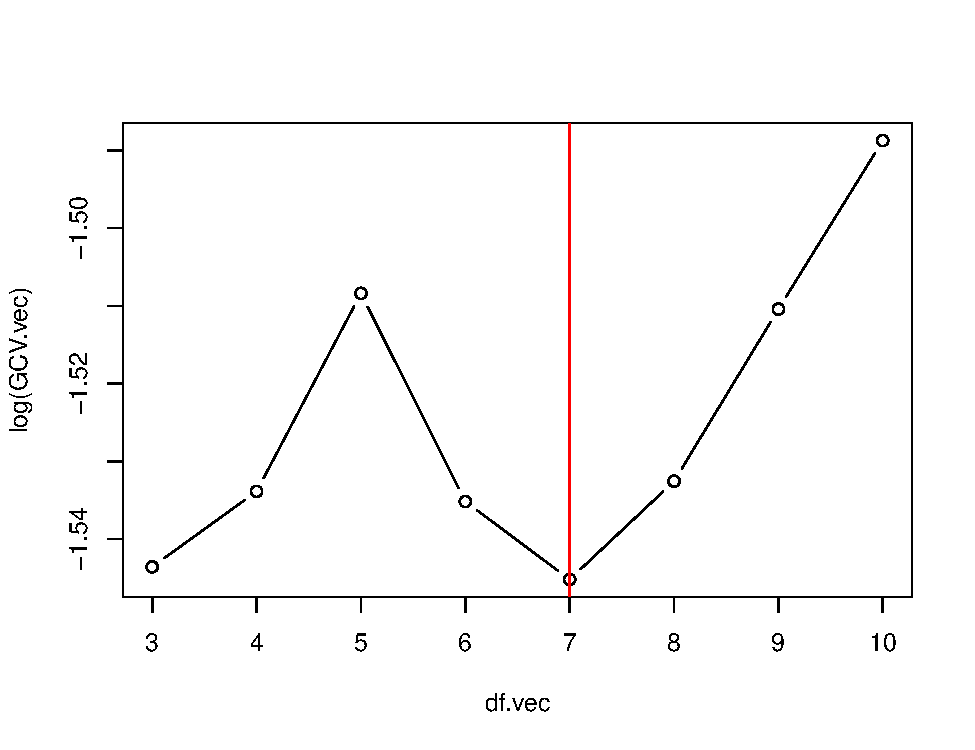
\includegraphics[width=\maxwidth]{figure/unnamed-chunk-12-1} 

}


\end{knitrout}

\textbf{R-Code} for computing the GCV-optimal fit:

\begin{knitrout}
\definecolor{shadecolor}{rgb}{0.878, 0.918, 0.933}\color{fgcolor}\begin{kframe}
\begin{alltt}
\hlstd{fit} \hlkwb{<-} \hlkwd{lm}\hlstd{(y_vec} \hlopt{~} \hlkwd{bs}\hlstd{(x_vec,}\hlkwc{df}\hlstd{=df.vec[}\hlkwd{which.min}\hlstd{(GCV.vec)]))}
\hlcom{## plot}
\hlkwd{plot}\hlstd{(}\hlkwc{y}\hlstd{=y_vec,} \hlkwc{x}\hlstd{=x_vec,} \hlkwc{xlab} \hlstd{=} \hlstr{"X"}\hlstd{,} \hlkwc{ylab} \hlstd{=} \hlstr{"Y"}\hlstd{)}
\hlkwd{lines}\hlstd{(}\hlkwc{y}\hlstd{=}\hlkwd{sin}\hlstd{(x_vec} \hlopt{*} \hlnum{5}\hlstd{),} \hlkwc{x}\hlstd{=x_vec,} \hlkwc{col}\hlstd{=}\hlstr{"red"}\hlstd{,} \hlkwc{lty}\hlstd{=}\hlnum{2}\hlstd{,} \hlkwc{lwd}\hlstd{=}\hlnum{1.5}\hlstd{)}
\hlkwd{lines}\hlstd{(}\hlkwc{x}\hlstd{=x_vec,} \hlkwc{y}\hlstd{=}\hlkwd{predict}\hlstd{(fit),} \hlkwc{col}\hlstd{=}\hlstr{"blue"}\hlstd{)}
\hlkwd{legend}\hlstd{(}\hlstr{"bottomleft"}\hlstd{,}
       \hlkwd{c}\hlstd{(}\hlstr{"(Unknown) Regression Function m"}\hlstd{,}
         \hlstr{"Regr.-Spline using GCV (p=7)"}\hlstd{),}
       \hlkwc{col}\hlstd{=}\hlkwd{c}\hlstd{(}\hlstr{"red"}\hlstd{,}\hlstr{"blue"}\hlstd{),}
       \hlkwc{lty}\hlstd{=}\hlkwd{c}\hlstd{(}\hlnum{2}\hlstd{,}\hlnum{1}\hlstd{),} \hlkwc{lwd}\hlstd{=}\hlkwd{c}\hlstd{(}\hlnum{2}\hlstd{,}\hlnum{2}\hlstd{))}
\end{alltt}
\end{kframe}

{\centering 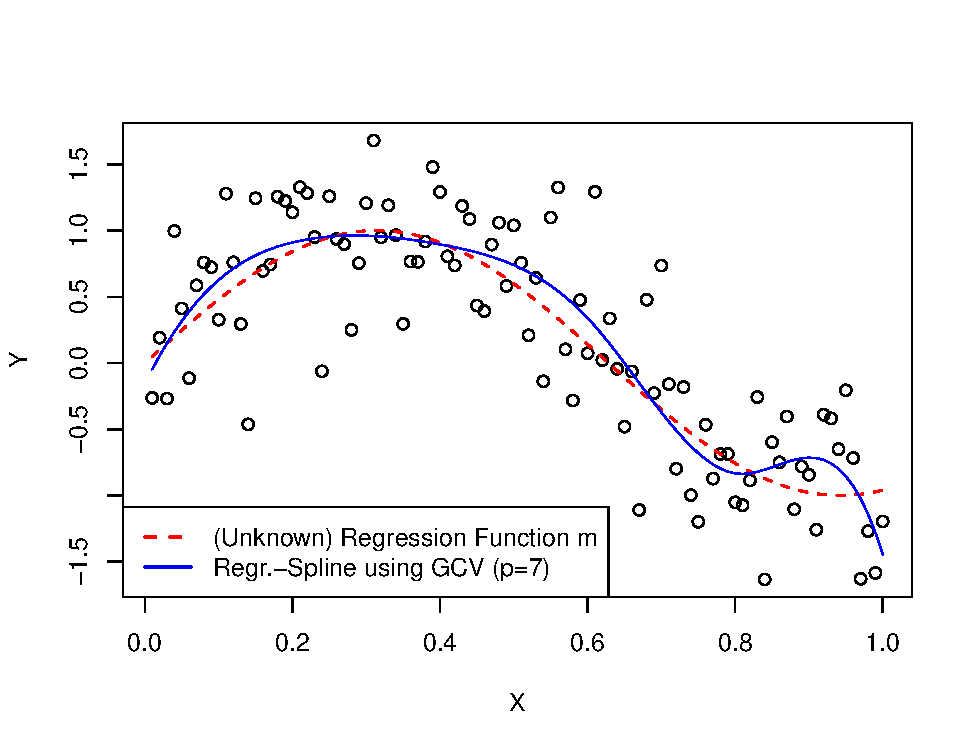
\includegraphics[width=\maxwidth]{figure/unnamed-chunk-13-1} 

}


\end{knitrout}


\newpage

\textbf{MARS-Algorithm:} 
There are more advanced procedures which estimate $p$ {\em as well as a best placement} of the
knots $\tau_1,\dots,\tau_q$ simultaneously from the data (MARS algorithm).



\begin{knitrout}
\definecolor{shadecolor}{rgb}{0.878, 0.918, 0.933}\color{fgcolor}\begin{kframe}
\begin{alltt}
\hlcom{## Multivariate Adaptive Regression Splines (MARS)}
\hlkwd{suppressMessages}\hlstd{(}\hlkwd{library}\hlstd{(}\hlstr{"earth"}\hlstd{))}
\end{alltt}


{\ttfamily\noindent\bfseries\color{errorcolor}{\#\# Error in library("{}earth"{}): there is no package called 'earth'}}\begin{alltt}
\hlstd{fit} \hlkwb{<-} \hlkwd{earth}\hlstd{(}\hlkwc{formula}\hlstd{=y_vec} \hlopt{~} \hlstd{x_vec)}
\end{alltt}


{\ttfamily\noindent\bfseries\color{errorcolor}{\#\# Error in earth(formula = y\_vec \textasciitilde{} x\_vec): could not find function "{}earth"{}}}\begin{alltt}
\hlcom{## plot}
\hlkwd{plot}\hlstd{(}\hlkwc{y}\hlstd{=y_vec,} \hlkwc{x}\hlstd{=x_vec,} \hlkwc{xlab} \hlstd{=} \hlstr{"X"}\hlstd{,} \hlkwc{ylab} \hlstd{=} \hlstr{"Y"}\hlstd{)}
\hlkwd{lines}\hlstd{(}\hlkwc{y}\hlstd{=}\hlkwd{sin}\hlstd{(x_vec} \hlopt{*} \hlnum{5}\hlstd{),} \hlkwc{x}\hlstd{=x_vec,} \hlkwc{col}\hlstd{=}\hlstr{"red"}\hlstd{,} \hlkwc{lty}\hlstd{=}\hlnum{2}\hlstd{,} \hlkwc{lwd}\hlstd{=}\hlnum{1.5}\hlstd{)}
\hlkwd{lines}\hlstd{(}\hlkwc{x}\hlstd{=x_vec,} \hlkwc{y}\hlstd{=}\hlkwd{predict}\hlstd{(fit),} \hlkwc{col}\hlstd{=}\hlstr{"blue"}\hlstd{)}
\hlkwd{legend}\hlstd{(}\hlstr{"bottomleft"}\hlstd{,}
\hlkwd{c}\hlstd{(}\hlstr{"(Unknown) Regression Function m"}\hlstd{,} \hlstr{"MARS-Algorithm"}\hlstd{),}
\hlkwc{col}\hlstd{=}\hlkwd{c}\hlstd{(}\hlstr{"red"}\hlstd{,}\hlstr{"blue"}\hlstd{),} \hlkwc{lty}\hlstd{=}\hlkwd{c}\hlstd{(}\hlnum{2}\hlstd{,}\hlnum{1}\hlstd{),} \hlkwc{lwd}\hlstd{=}\hlkwd{c}\hlstd{(}\hlnum{2}\hlstd{,}\hlnum{2}\hlstd{))}
\end{alltt}
\end{kframe}

{\centering 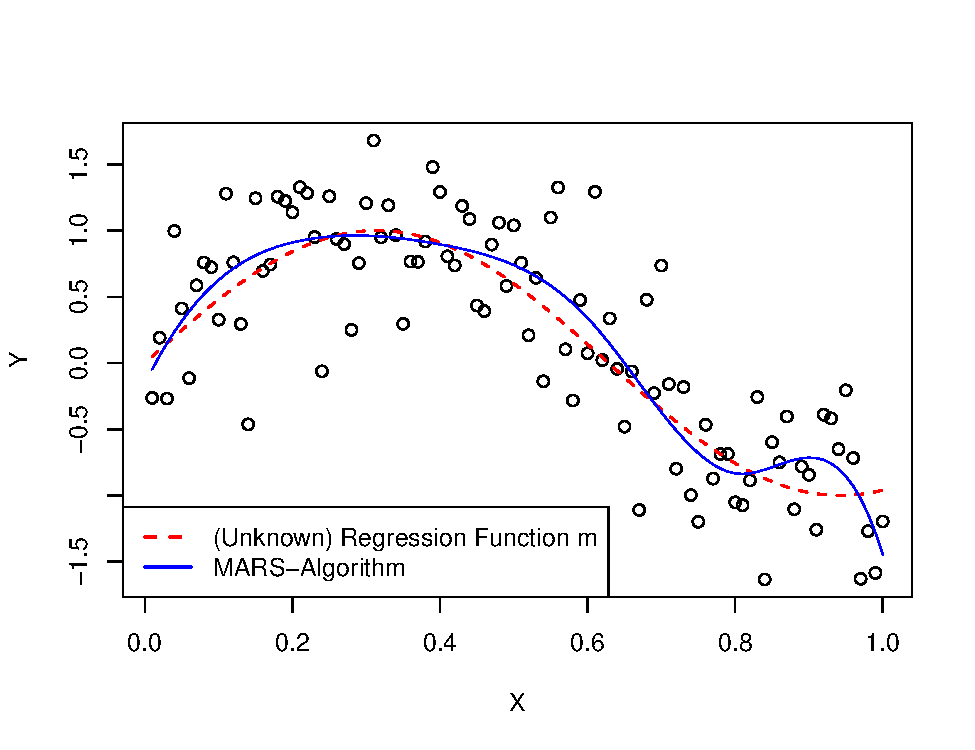
\includegraphics[width=\maxwidth]{figure/unnamed-chunk-14-1} 

}


\end{knitrout}

\newpage

\subsection{Approaches Based on Roughness Penalties}

A different approach to spline fitting, which is widely used in practice, is based on the use of
a \emph{roughness penalty}. The basic idea can be described as follows:
\begin{itemize}
\item In order to guarantee a small systematic error, spline functions are defined with respect to
 a large number of knots ($\frac{p}{n}$ close to 1).
\item Variability of the estimator is controlled by fitting the coefficients subject to a
 penalty which penalizes roughness (non-smoothness) of the resulting function. A convenient measure
 of smoothness is $\int_a^b m''(x)^2dx$.
\end{itemize}


\bigskip
\bigskip

\textbf{Smoothing Splines}

\bigskip

The so-called  ''(cubic) smoothing spline approach'' relies on cubic splines with knots at each observation
point. More precisely:
\begin{itemize}
\item $q=n$ and 
\item $\tau_1=X_1,\tau_2=X_2,\dots,\tau_n=X_n$. 
\item The side conditions $s''(a)=0$ and $s''(b)=0$
are additionally imposed in order to ensure that the number of coefficients to be estimated is equal to the sample size, i.e., that $p=n$.
\end{itemize}

\bigskip

In the following we will consider cubic splines ($k=3$). For a \textbf{smoothing parameter} $\lambda>0$ (to be selected by the statistician), an estimate $\hat m_\lambda(x)=\sum_j\hat\beta_j b_j(x)$ is determined by
\begin{align*}
&\frac{1}{n} \sum_i (Y_i-\hat m_\lambda(X_i))^2+\lambda \int_a^b \hat m_\lambda''(x)^2dx\\ &=
\min_{s\in {\cal{S}}_{3,\tau_1,\dots,\tau_q}}\left\{\frac{1}{n} \sum_i (Y_i-s(X_i))^2+\lambda \int_a^b s''(x)^2dx\right\},\end{align*}
or equivalently,
\begin{align*}
&\frac{1}{n} \sum_i (Y_i-\sum_j \hat\beta_j b_j(X_i))^2+\lambda \int_a^b (\sum_j \hat\beta_j b_j''(x))^2dx\\
&=\min_{\vartheta_1,\dots,\vartheta_p}\left\{ \frac{1}{n}
 \sum_i (Y_i-\sum_j\vartheta_j b_j(X_i))^2+\lambda \int_a^b (\sum_j \vartheta_j b_j''(x))^2dx\right\}.
\end{align*}

\bigskip

Let $\mathbf{X}$  denote the $n\times p$ matrix with elements $b_j(X_i)$, and let $\mathbf{B}$ denote the $p\times p$ matrix
with elements $n \int_a^b b_j''(x)b_l''(x)dx$, $j,l=1,\dots,p$. Then the solutions are given by
$$\hat\beta =(\mathbf{X}^\top \mathbf{X}+\lambda \mathbf{B})^{-1}\mathbf{X}^\top Y, \quad
\hat m_\lambda = \underbrace{\mathbf{X}(\mathbf{X}^\top \mathbf{X}+\lambda \mathbf{B})^{-1}\mathbf{X}^\top }_{S_\lambda}Y,$$
where $\hat m_\lambda=(\hat m_\lambda(X_1),\dots,\hat m_\lambda(X_n))^\top $.

\bigskip

Here only the choice of the \textbf{smoothing parameter} $\lambda$ is crucial for the quality of the estimator. Let's take a look at the effect of $\lambda$. First, we need some data:
\begin{knitrout}
\definecolor{shadecolor}{rgb}{0.878, 0.918, 0.933}\color{fgcolor}\begin{kframe}
\begin{alltt}
\hlkwd{set.seed}\hlstd{(}\hlnum{1}\hlstd{)}
\hlcom{# Generate some data: ####################################}
\hlstd{n}      \hlkwb{<-} \hlnum{100}     \hlcom{# Sample Size}
\hlstd{x_vec}  \hlkwb{<-} \hlstd{(}\hlnum{1}\hlopt{:}\hlstd{n)}\hlopt{/}\hlstd{n} \hlcom{# Equidistant X }
\hlcom{# Gaussian iid error term }
\hlstd{e_vec}  \hlkwb{<-} \hlkwd{rnorm}\hlstd{(}\hlkwc{n} \hlstd{= n,} \hlkwc{mean} \hlstd{=} \hlnum{0}\hlstd{,} \hlkwc{sd} \hlstd{=} \hlnum{.5}\hlstd{)}
\hlcom{# Dependent variable Y}
\hlstd{y_vec}  \hlkwb{<-}  \hlkwd{sin}\hlstd{(x_vec} \hlopt{*} \hlnum{5}\hlstd{)} \hlopt{+} \hlstd{e_vec}
\hlcom{#########################################################}
\end{alltt}
\end{kframe}
\end{knitrout}

\bigskip

Below we use the pre-installed smoothing spline function of R, bu there are many R-packages that contain routines for computing smoothing-splines (see, e.g., \texttt{library(pspline)}). 
\begin{knitrout}
\definecolor{shadecolor}{rgb}{0.878, 0.918, 0.933}\color{fgcolor}\begin{kframe}
\begin{alltt}
\hlstd{lambda.1} \hlkwb{<-} \hlnum{0.1}
\hlstd{sm.spl.1} \hlkwb{<-} \hlkwd{smooth.spline}\hlstd{(}\hlkwc{x}\hlstd{=x_vec,} \hlkwc{y}\hlstd{=y_vec,} \hlkwc{all.knots}\hlstd{=}\hlnum{TRUE}\hlstd{,}
                          \hlkwc{spar} \hlstd{= lambda.1)}
\hlstd{lambda.2} \hlkwb{<-} \hlnum{0.9}
\hlstd{sm.spl.2} \hlkwb{<-} \hlkwd{smooth.spline}\hlstd{(}\hlkwc{x}\hlstd{=x_vec,} \hlkwc{y}\hlstd{=y_vec,} \hlkwc{all.knots}\hlstd{=}\hlnum{TRUE}\hlstd{,}
                          \hlkwc{spar} \hlstd{= lambda.2)}
\end{alltt}
\end{kframe}
\end{knitrout}

\newpage

Let's plot the results:
\begin{knitrout}
\definecolor{shadecolor}{rgb}{0.878, 0.918, 0.933}\color{fgcolor}\begin{kframe}
\begin{alltt}
\hlkwd{plot}\hlstd{(}\hlkwc{y}\hlstd{=y_vec,} \hlkwc{x}\hlstd{=x_vec,} \hlkwc{xlab}\hlstd{=}\hlstr{"X"}\hlstd{,} \hlkwc{ylab}\hlstd{=}\hlstr{"Y"}\hlstd{,}
    \hlkwc{main}\hlstd{=}\hlstr{"Smoothing Splines"}\hlstd{)}
\hlkwd{lines}\hlstd{(}\hlkwc{y}\hlstd{=}\hlkwd{sin}\hlstd{(x_vec} \hlopt{*} \hlnum{5}\hlstd{),} \hlkwc{x}\hlstd{=x_vec,} \hlkwc{col}\hlstd{=}\hlstr{"red"}\hlstd{,} \hlkwc{lty}\hlstd{=}\hlnum{2}\hlstd{,} \hlkwc{lwd}\hlstd{=}\hlnum{1.5}\hlstd{)}
\hlkwd{lines}\hlstd{(sm.spl.1,} \hlkwc{col}\hlstd{=}\hlstr{"blue"}\hlstd{,}       \hlkwc{lwd}\hlstd{=}\hlnum{1.5}\hlstd{)}
\hlkwd{lines}\hlstd{(sm.spl.2,} \hlkwc{col}\hlstd{=}\hlstr{"darkorange"}\hlstd{,} \hlkwc{lwd}\hlstd{=}\hlnum{1.5}\hlstd{)}
\hlkwd{legend}\hlstd{(}\hlstr{"bottomleft"}\hlstd{,}
      \hlkwd{c}\hlstd{(}\hlstr{"(Unknown) Regression Function"}\hlstd{,}
        \hlstr{"Sm.Spline Fit with spar=0.1"}\hlstd{,}
        \hlstr{"Sm.Spline Fit with spar=0.9"}\hlstd{),}
      \hlkwc{col}\hlstd{=}\hlkwd{c}\hlstd{(}\hlstr{"red"}\hlstd{,}\hlstr{"blue"}\hlstd{,} \hlstr{"darkorange"}\hlstd{),}
      \hlkwc{lty}\hlstd{=}\hlkwd{c}\hlstd{(}\hlnum{2}\hlstd{,}\hlnum{1}\hlstd{,}\hlnum{1}\hlstd{),} \hlkwc{lwd}\hlstd{=}\hlkwd{c}\hlstd{(}\hlnum{2}\hlstd{,}\hlnum{2}\hlstd{,}\hlnum{2}\hlstd{))}
\end{alltt}
\end{kframe}

{\centering 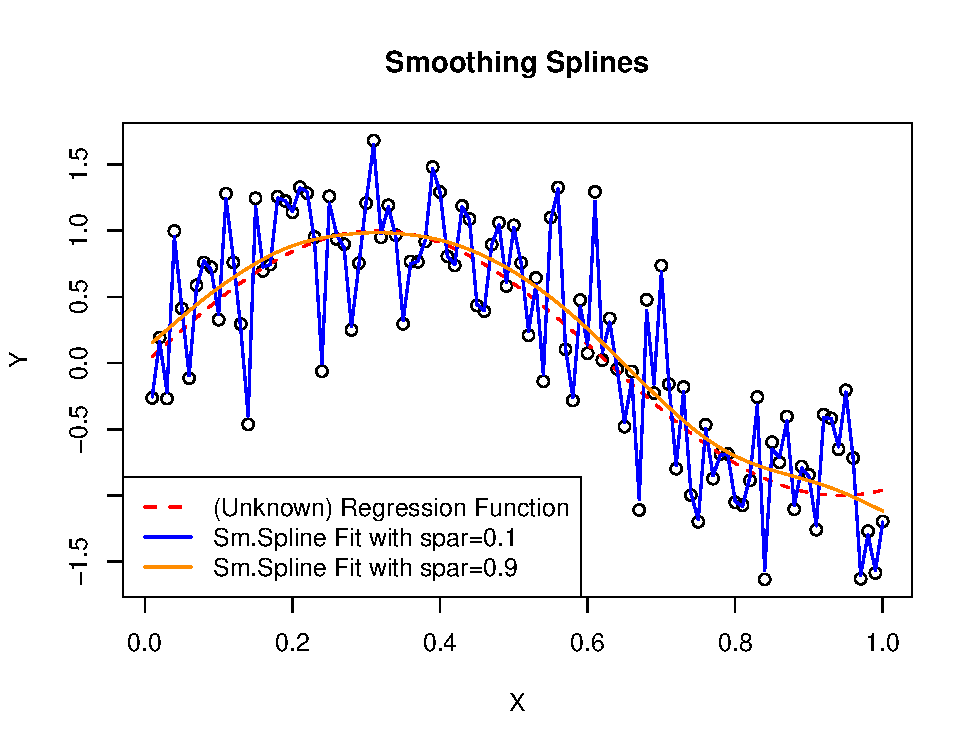
\includegraphics[width=\maxwidth]{figure/unnamed-chunk-17-1} 

}


\end{knitrout}

% 
% 
% \begin{center}
% \begin{tabular}{cc}
% \epsfig{ file=/Pics/chap1/pen1.ps, width=5cm,height=5cm} &
% \epsfig{ file=/Pics/chap1/pen2.ps, width=5cm,height=5cm}\\
% $\int  (m''(x))^2dx$ small & $\int  (m''(x))^2dx$ large
% \end{tabular}
% \end{center}
% \newslide
% 
% In the following we will concentrate on the situation that $p$ is large compared to $n$ (e.g. $p\approx n$) such that
% the bias of spline approximation is negligible. 

\newpage
\textbf{Bias, Variance and MASE}

\bigskip


The typical bias variance trade-off arises:
\begin{itemize}
\item $(\operatorname{Bias}(\hat m_\lambda))^2$ \emph{increases} as $\lambda$ increases.\\
Extreme case: $\lambda=\infty$ $\Rightarrow$ straight line fit.
\item $\V(\hat m_\lambda)$  \emph{decreases} as $\lambda$ increases. As a consequence, the estimated functions $\hat m_\lambda$ become the smoother the larger $\lambda$ is.
\end{itemize}

\bigskip

In the following, we will additionally assume that the true regression function $m$ is twice continuously differentiable. 
\bigskip
 
An optimal smoothing parameter $\lambda_{opt}$ will again balance bias and variance.
\begin{itemize}
\item It can be verified that
$$\frac{1}{n}\sum_i \V_\epsilon(\hat m_\lambda(X_i))=\frac{1}{n}\E_\epsilon\left(\epsilon^\top S_\lambda^2\epsilon\right)
=\frac{\sigma^2}{n}\operatorname{trace}(S_\lambda^2)$$
\item And that, as $n\rightarrow\infty$, $n\lambda\rightarrow \infty$,
$$\operatorname{trace}(S_\lambda^2)=O_p\left(\frac{1}{\lambda^{1/4}}\right)$$
% \item The ''degrees of freedoms'' of the estimation procedure are defined as $\operatorname{df}_\lambda=\operatorname{trace}(S_\lambda)$ (sometimes also
% $\operatorname{df}_\lambda^*=\operatorname{trace}(S_\lambda^2)$ is considered). These degrees of freedom can be seen as a nonparametric equivalent of the ''number of parameters to estimate'' in parametric regression.
\item For a twice continuously differential function $m$ it can be shown that $(\operatorname{Bias}(\hat m_\lambda))^2$ is proportional to $\lambda$.
\end{itemize}

% Let
% $$\tilde m_{\lambda}=(\tilde m_{\lambda}(X_1),\dots,\tilde m_\lambda(X_n))^\top =\E_\epsilon\left( S_\lambda Y\right)=
% \mathbf{X}(\mathbf{X}^\top \mathbf{X}+\lambda \mathbf{B})^{-1}\mathbf{X}^\top m$$
% 
% It is then easily seen that $\tilde m_{\lambda}$ is a solution of
% \begin{align*}
% &\frac{1}{n} \sum_i (m(X_i)-\tilde m_\lambda(X_i))^2+\lambda \int_a^b \tilde m_\lambda''(x)^2dx\\ &=
% \min_{s\in {\cal{S}}_{k,\tau_1,\dots,\tau_q}}\left\{\frac{1}{n} \sum_i (m(X_i)-s(X_i))^2+\lambda \int_a^b s''(x)^2dx\right\}\end{align*}
% 
% 
% If the number of knots is sufficiently large, then the bias of a {\bf best} possible spline approximation $s_{opt}\in  {\cal{S}}_{3,\tau_1,\dots,\tau_q}$ to $m$
%  is negligible, i.e.,
% $m\approx s_{opt}$. The above relation then implies that for large number of knots
% $$\frac{1}{n} \sum_i (m(X_i)-\tilde m_\lambda(X_i))^2+\lambda \int_a^b \tilde m_\lambda''(x)^2dx\le \lambda \int_a^b  m''(x)^2dx$$
% For a twice continuously differential function $m$ it can indeed be shown that $Bias(\hat m_\lambda)^2$ is
% proportional to $\lambda$.
 
Hence, as $n\rightarrow\infty$, $\lambda\rightarrow 0$, $n\lambda\rightarrow\infty$,
$$\operatorname{MASE}(\hat m_{\lambda})=O_p\left(\lambda +\frac{1}{n\lambda^{1/4}}\right),$$

which implies that an optimal smoothing parameter balancing bias and variance will be of order $\lambda_{opt}\sim n^{-4/5}$. Then
$$\operatorname{MASE}(\hat m_{\lambda_{opt}})=O_p(n^{-4/5}).$$


% Similar results can be obtained for the mean integrated squared error (MISE):
% $$\operatorname{MISE}(\hat m)=\E_\epsilon\left(\int_a^b(m(x)-\hat m_{\lambda_{opt}}(x))^2dx\right)=O_p(n^{-4/5})$$

\bigskip

Again, estimates of $\lambda_{opt}$ may be determined by minimizing $\operatorname{CV}(\lambda)$ or $\operatorname{GCV}(\lambda)$:

\begin{itemize}
\item {\bf Cross-validation (CV)}:
$$\operatorname{CV}(\lambda)={1 \over n} \sum_{i=1}^n\biggl( Y_i-
{\hat m}_{\lambda,-i}(X_i)\biggr)^2,$$
Here, for any $i=1,\dots,n$, ${\hat m}_{p,-i}$ is the ''leave-one-out'' estimator of
$m$ to be obtained when only the $n-1$
observations\\
$(Y_1,X_1),\dots,(Y_{i-1},X_{i-1}),(Y_{i+1},X_{i+1}),\dots,
(Y_{n},X_{n})$ are used.
\item {\bf Generalized cross-validation (GCV)}:
$$\operatorname{GCV}(\lambda)={1\over n\Big(1-{df_\lambda\over n}\Big)^2}\sum_{i=1}^n \biggl( Y_i-
{\hat m}_\lambda(X_i)\biggr)^2,$$
where $\operatorname{df}_\lambda:=\operatorname{trace}(S_\lambda)$ ($=$ degrees of freedom)
\end{itemize}

The ''degrees of freedoms'' of the estimation procedure are defined as $\operatorname{df}_\lambda=\operatorname{trace}(S_\lambda)$ (sometimes also $\operatorname{df}_\lambda^*=\operatorname{trace}(S_\lambda^2)$ is considered). These degrees of freedom can be seen as a nonparametric equivalent of the ''number of parameters to estimate'' in parametric regression.

\bigskip
\bigskip

The R-function $\texttt{smooth.spline}$ has build-in routines for CV and GCV:
\begin{knitrout}
\definecolor{shadecolor}{rgb}{0.878, 0.918, 0.933}\color{fgcolor}\begin{kframe}
\begin{alltt}
\hlstd{sm.spl.cv}  \hlkwb{<-} \hlkwd{smooth.spline}\hlstd{(}\hlkwc{x}\hlstd{=x_vec,}\hlkwc{y}\hlstd{=y_vec,}\hlkwc{all.knots}\hlstd{=}\hlnum{TRUE}\hlstd{,}
                            \hlkwc{cv}\hlstd{=}\hlnum{TRUE}\hlstd{)}
\hlstd{sm.spl.gcv} \hlkwb{<-} \hlkwd{smooth.spline}\hlstd{(}\hlkwc{x}\hlstd{=x_vec,}\hlkwc{y}\hlstd{=y_vec,}\hlkwc{all.knots}\hlstd{=}\hlnum{TRUE}\hlstd{,}
                            \hlkwc{cv}\hlstd{=}\hlnum{FALSE}\hlstd{)}
\end{alltt}
\end{kframe}
\end{knitrout}

\newpage

Let's plot the results:
\begin{knitrout}
\definecolor{shadecolor}{rgb}{0.878, 0.918, 0.933}\color{fgcolor}\begin{kframe}
\begin{alltt}
\hlkwd{plot}\hlstd{(}\hlkwc{y}\hlstd{=y_vec,} \hlkwc{x}\hlstd{=x_vec,} \hlkwc{xlab}\hlstd{=}\hlstr{"X"}\hlstd{,} \hlkwc{ylab}\hlstd{=}\hlstr{"Y"}\hlstd{,}
    \hlkwc{main}\hlstd{=}\hlstr{"Smoothing Splines"}\hlstd{)}
\hlkwd{lines}\hlstd{(}\hlkwc{y}\hlstd{=}\hlkwd{sin}\hlstd{(x_vec} \hlopt{*} \hlnum{5}\hlstd{),} \hlkwc{x}\hlstd{=x_vec,} \hlkwc{col}\hlstd{=}\hlstr{"red"}\hlstd{,} \hlkwc{lty}\hlstd{=}\hlnum{2}\hlstd{,} \hlkwc{lwd}\hlstd{=}\hlnum{1.5}\hlstd{)}
\hlkwd{lines}\hlstd{(sm.spl.cv,}  \hlkwc{col}\hlstd{=}\hlstr{"blue"}\hlstd{,}       \hlkwc{lwd}\hlstd{=}\hlnum{4.5}\hlstd{)}
\hlkwd{lines}\hlstd{(sm.spl.gcv,} \hlkwc{col}\hlstd{=}\hlstr{"darkorange"}\hlstd{,} \hlkwc{lwd}\hlstd{=}\hlnum{1.5}\hlstd{)}
\hlkwd{legend}\hlstd{(}\hlstr{"bottomleft"}\hlstd{,}
      \hlkwd{c}\hlstd{(}\hlstr{"(Unknown) Regression Function"}\hlstd{,}
        \hlstr{"Sm.Spline Fit using CV"}\hlstd{,}
        \hlstr{"Sm.Spline Fit using GCV"}\hlstd{),}
      \hlkwc{col}\hlstd{=}\hlkwd{c}\hlstd{(}\hlstr{"red"}\hlstd{,}\hlstr{"blue"}\hlstd{,} \hlstr{"darkorange"}\hlstd{),}
      \hlkwc{lty}\hlstd{=}\hlkwd{c}\hlstd{(}\hlnum{2}\hlstd{,}\hlnum{1}\hlstd{,}\hlnum{1}\hlstd{),} \hlkwc{lwd}\hlstd{=}\hlkwd{c}\hlstd{(}\hlnum{2}\hlstd{,}\hlnum{3}\hlstd{,}\hlnum{2}\hlstd{))}
\end{alltt}
\end{kframe}

{\centering 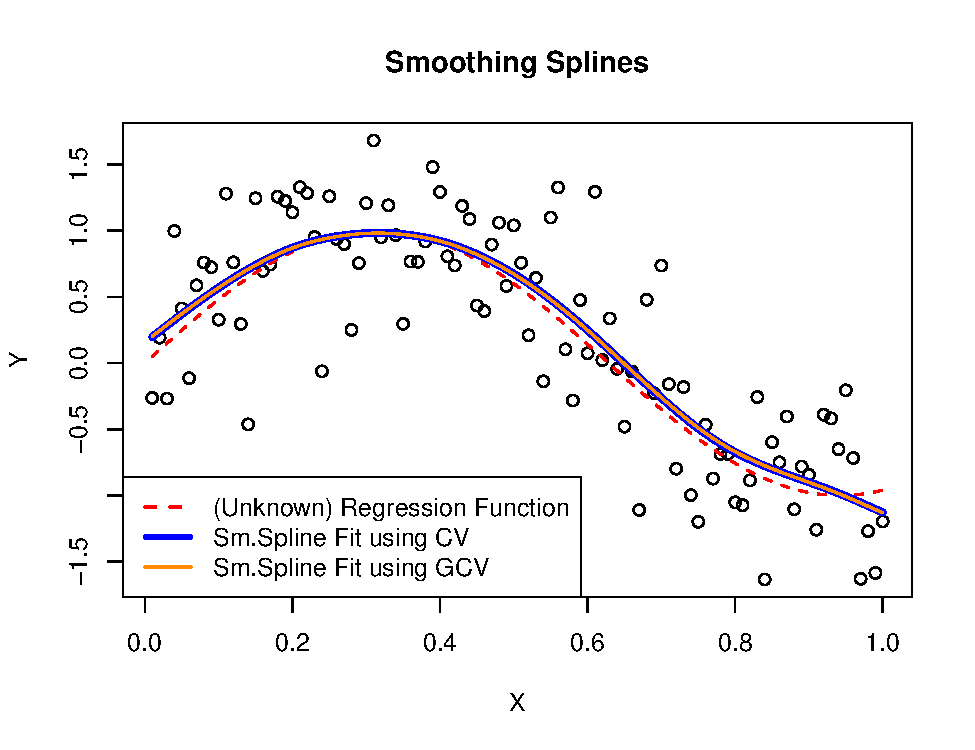
\includegraphics[width=\maxwidth]{figure/unnamed-chunk-19-1} 

}


\end{knitrout}



% {\em Remark:} Under some regularity conditions it can be shown that
% $$MASE(\hat m_{\lambda_{opt}})-MASE(\hat m_{\hat\lambda_{opt}})=O_P\left(n^{-1/2} MASE(\hat m_{\lambda_{opt}})^{1/2}\right),$$
% where $\hat\lambda_{opt}$ denotes the smoothing parameters estimated by CV or GCV.
% 
% \end{slide*}
% \begin{slide*}
%  Smoothing Splines ($df_ h=3$)
% \begin{center}
% \epsfig{ file=/Pics/chap1/spline3.eps, width=10cm,height=6cm} \end{center}
% \bigbreak\noindent
% 
% \begin{center} Smoothing Splines ($df_ h=10$) \epsfig{ file=/Pics/chap1/spline10.eps,
% width=10cm,height=6cm} \end{center}
% \end{slide*}
% \begin{slide*}
% 
% 
% \subsection{ Estimating the error variance}
% \bigbreak\noindent
% The magnitude of the variance $\sigma^2$ of the error terms $\epsilon_i$ influences the accuracy of the estimators. For
% simplicity it will in the following be assumed that the observations $X_i$ are ordered,
%  $X_1\le X_2\le\dots\le X_n$, and that $m$ is a smooth,
% twice continuously differentiable function.
% 
% \begin{itemize}
% \item[a)] Based on an nonparametric estimate $\hat m$ of $m$ a simple estimate of $\sigma^2$ is obtained by averaging
% squared residuals:
% $$\hat\sigma^2:= \frac{1}{n}\sum_i (Y_i-\hat m(X_i))^2$$
% \item[b)] The method of Rice:
% $$\hat \sigma^2: =\frac{1}{2(n-1)} \sum_{i=2}^n (Y_i-Y_{i-1})^2$$
% It can be shown that $E_\epsilon(\hat\sigma^2)=\sigma^2+O_P(\frac{1}{n^2})$ and $Var_\epsilon(\hat\sigma^2)=O_P(\frac{1}{n})$.
% \item[c)] The method of Gasser et.al.: In a first step
%   ''pseudo-residuals''
% $$\hat\epsilon_i=\frac{X_{i+1}-X_i}{X_{i+1}-X_{i-1}}Y_{i-1}+\frac{X_i-X_{i-1}}{X_{i+1}-X_{i-1}}Y_{i+1}-Y_i$$
% are calculated. Then
% $$\hat \sigma^2: =\frac{1}{n-2} \sum_{i=2}^{n-1} \hat\epsilon_i^2$$
% \end{itemize}
% Often methods b) or c) are preferred to a). The important point is that the bias of the estimators in b) or c) is much smaller
% than the bias of the estimator in a). However, all procedures a), b), c) yield consistent estimators of $\sigma^2$.
% 
% \newslide
% \centerline{{\large\bf Confidence Intervals for spline methods}}
% \bigbreak
% Consider spline fitting based on a roughness penalty with smoothing parameter $\lambda$.
% Under some suitable regularity conditions
% it can easily be shown that as $n\rightarrow\infty$, $\lambda\rightarrow 0$, $n\lambda\rightarrow\infty$,
% $$\frac{\hat m_\lambda(x) -\tilde m_\lambda(x)}{\sqrt{var_\epsilon(\hat m_\lambda(x))}}\rightarrow_L N(0,1)$$
% holds for all $x$ (central limit theorem).\\ Here again
%  $\tilde m_\lambda(x)=E_\epsilon(\hat m_\lambda(x))$.
% 
%  Note that with
%  $$cov_\epsilon(\hat\beta)=\sigma^2\left(
%  \underbrace{(\mathbf{X}^\top \mathbf{X}+\lambda \mathbf{B})^{-1}\mathbf{X}^\top \mathbf{X}(\mathbf{X}^\top \mathbf{X}+\lambda \mathbf{B})^{-1}}_{Q_\lambda}\right)$$
%  This implies that with $b(x)=(b_1(x),\dots,b_p(x))^\top $
%  $$var_\epsilon(\hat m_\lambda(x))=var_\epsilon(b(x)^\top \hat\beta) =\sigma^2 b(x)^\top Q_\lambda b(x).$$
% 
%  Based on an estimate $\hat\sigma^2$ of $\sigma^2$ this leads to asymptotically valid  $(1-\alpha)$ confidence intervals for
%  $\tilde m_h(x)$:
% $$\hat m_h(x)\pm z_{1-\alpha/2}\sqrt{\hat\sigma^2 b(x)^\top Q_\lambda b(x)},$$
% where $z_{1-\alpha/2}$ is the $1-\alpha/2$-quantile of the standard normal distribution (e.g. $z_{0.0975}=1.96$).
% 
% These intervals can be calculated for any point $x$ $\Rightarrow$ confidence bands for the function $\tilde m_h$.
% 
% In the literature one speaks of confidence intervals for the  ''variability'' of $\hat m_\lambda(x)$ (i.e.
% error bounds for the random fluctuation due to the error terms $\ep_i$). Quite obviously, bias is
%  {\em not} taken into account when calculating these intervals.
% 
% \end{slide*}
% 
% \begin{slide*}


\newpage

\subsection{The Nadaraya-Watson Kernel Estimator}

\bigbreak\noindent {\bf General Idea:} Approximation of $m(x)$ by a local average of the
 observations $Y_i$:
$${\hat m}_ h(x)=\sum_{i=1}^n w(x,X_i, h)Y_i$$
\begin{itemize}
\item The weight function
$w$ is constructed in such a way that the weight of an  observation $Y_i$ is the smaller the larger the distance
$|x-X_i|$. A smoothing parameter (''bandwidth'')
$h$ determines the rate of decrease of the weights $w(x,X_i, h)$ as
$|x-X_i|$ increases.
\end{itemize}
\par\noindent
\textbf{Kernel estimators} calculate weights on the basis of a pre-specified
\textbf{kernel function} $K$. Usually  $K$ is chosen as a symmetric density function.
 
\bigbreak
 
\par\noindent
{\bf Nadaraya-Watson (NW) kernel estimator}:
%$${\hat m}_ h(x)={\sum_{i=1}^n K({x-X_i\over h})Y_i\over
%\sum_{i=1}^n K({x-X_i\over h})}$$
\begin{align*}
{\hat m}_ h(x)&=\sum_{i=1}^n {K({x-X_i\over h})\over
\sum_{j=1}^n K({x-X_j\over h})}Y_i\\[2ex]
&=\frac{\frac{1}{nh} \sum_{i=1}^n K({x-X_i\over h})Y_i}{
\frac{1}{nh} \sum_{j=1}^n K({x-X_j\over h})}
\end{align*}
 
Some properties:
\begin{itemize}
\item For every possible bandwidth $h>0$ the sum of all weights
$$
w(x,X_i, h)=K\Big({x-X_i\over h}\Big)/\sum_{j=1}^n
K\Big({x-X_j\over h}\Big)
$$
is always equal to 1, i.e., $\sum_i w(x,X_i, h)=1$.

\item Kernel estimators are \textbf{linear} smoothing methods:
$$
\hat m_h=(\hat m_h(X_1),\dots,\hat m_h(X_n))^T=S_h Y,
$$
where the elements of the $n\times n$ matrix
$S_ h$ are given by
$$
(S_ h)_{ij}={ K\Big({X_i-X_j\over  h}\Big)\over
\sum_{l=1}^n K\Big({X_i-X_l\over h}\Big)},\quad\text{and where }\;\operatorname{trace}(S_h)=O\left(\frac{1}{h}\right).
$$
\end{itemize}

\bigskip

Similar to density estimation, usually second-order kernel functions are used in practice.
The most important examples are:
\begin{itemize}
\item Epanechnikov kernel
% $$K(x)=\left\{
% \begin{array}{ll}
% {3\over 4} (1-x^2) & \hbox{ if } |x|\le 1\\
% 0& \hbox{ if } |x|> 1\end{array}\right.$$
\item Gaussian kernel
%$$K(x)={1\over \sqrt{2\pi}} \exp(-x^2/2)$$
\item Biweight (quartic) kernel
% $$K(x)=\left\{
% \begin{array}{ll}
% \frac{15}{16} (1-x^2)^2 & \hbox{ if } |x|\le 1\\
%  0& \hbox{ if } |x|> 1\end{array}\right.$$
\end{itemize}

\bigskip

% \textbf{Theoretical Justification of the NW Kernel Estimator}:\\
% 
% Assume that $m$ is a continuous function.
% Under random design, as $n\rightarrow\infty$, $h\rightarrow 0$ and $nh\rightarrow \infty$
% %{\small
% \begin{align*}
% \frac{1}{nh} \sum_{i=1}^n K({x-X_i\over h})Y_i&=
% \frac{1}{nh} \sum_{i=1}^n K({x-X_i\over h})m(X_i)+\frac{1}{nh} \sum_{i=1}^n K({x-X_i\over h})\epsilon_i\\
% &=\int_{-\infty}^\infty  \frac{1}{h} K({x-u\over h})m(u)f(u)du+o_p(1)\\
% &=m(x)f(x)+o_p(1),
% \end{align*}
% %}
% while $\frac{1}{nh} \sum_{j=1}^n K({x-X_j\over h})\rightarrow_p f(x)$. Hence,
% $${\hat m}_ h(x)\rightarrow_P \frac{m(x)f(x)}{f(x)}=m(x)$$





%' % 
%' % \begin{slide*}
%' % \begin{center}
%' % \epsfig{ file=/Pics/chap1/fig2.eps, width=10cm,height=6cm}
%' % \end{center}
%' \begin{itemize}
%' \item $ h$ small $\quad \Rightarrow$  $\hat m_h(x)$ is determined by averaging over
%'  {\bf few} observations $Y_i$
%' $\quad \Rightarrow$ small bias, large variance.
%' \item $ h$ large $\quad \Rightarrow$ averaging over
%' {\bf many} observation $Y_i$.
%' $\quad \Rightarrow$ small variance, but possibly large bias.
%' \item Minimizing $\operatorname{CV}(h)$ or $\operatorname{GCV}(h)$ provides an appropriate way to estimate an optimal bandwidth $h$;
%' $\operatorname{df}_h=\operatorname{trace}(S_h)$ is proportional to ${1\over h}$.
%' \end{itemize}
%' 
R-Code for computing the NW-Estimator:\\
First generate some data.
\begin{knitrout}
\definecolor{shadecolor}{rgb}{0.878, 0.918, 0.933}\color{fgcolor}\begin{kframe}
\begin{alltt}
\hlcom{# Generate some data: ###############################}
\hlcom{# Equidistant X }
\hlstd{n}      \hlkwb{<-} \hlnum{100}
\hlstd{x_vec}  \hlkwb{<-} \hlstd{(}\hlnum{1}\hlopt{:}\hlstd{n)}\hlopt{/}\hlstd{n}
\hlcom{# Gaussian iid error term }
\hlstd{e_vec}  \hlkwb{<-} \hlkwd{rnorm}\hlstd{(}\hlkwc{n} \hlstd{= n,} \hlkwc{mean} \hlstd{=} \hlnum{0}\hlstd{,} \hlkwc{sd} \hlstd{=} \hlnum{.5}\hlstd{)}
\hlcom{# Dependent variable Y}
\hlstd{y_vec}  \hlkwb{<-}  \hlkwd{sin}\hlstd{(x_vec} \hlopt{*} \hlnum{5}\hlstd{)} \hlopt{+} \hlstd{e_vec}
\hlcom{# Save all in a dataframe}
\hlstd{db}     \hlkwb{<-}  \hlkwd{data.frame}\hlstd{(}\hlkwc{x}\hlstd{=x_vec,}\hlkwc{y}\hlstd{=y_vec)}
\end{alltt}
\end{kframe}
\end{knitrout}

%\newpage
Choose a kernel function (e.g., the Epanechnikov kernel) and write a function for the weights $w(x,X_i,h)$:
\begin{knitrout}
\definecolor{shadecolor}{rgb}{0.878, 0.918, 0.933}\color{fgcolor}\begin{kframe}
\begin{alltt}
\hlcom{# Epanechnikov kernel function}
\hlstd{epanech_kern_f}   \hlkwb{<-} \hlkwa{function}\hlstd{(}\hlkwc{u}\hlstd{)\{}
   \hlkwd{ifelse}\hlstd{(}\hlkwd{abs}\hlstd{(u)}\hlopt{<=}\hlnum{1}\hlstd{,(}\hlnum{3}\hlopt{/}\hlnum{4}\hlstd{)}\hlopt{*}\hlstd{(}\hlnum{1}\hlopt{-}\hlstd{u}\hlopt{^}\hlnum{2}\hlstd{),} \hlnum{0}\hlstd{)\}}

\hlcom{# Function to compute the kernel-weights:}
\hlstd{w_fun} \hlkwb{<-} \hlkwa{function}\hlstd{(}\hlkwc{x0}\hlstd{,} \hlkwc{x_vec}\hlstd{,} \hlkwc{h}\hlstd{)\{}
   \hlstd{u}     \hlkwb{<-} \hlstd{(x_vec} \hlopt{-} \hlstd{x0)}\hlopt{/}\hlstd{h}
   \hlstd{epa_w} \hlkwb{<-} \hlkwd{epanech_kern_f}\hlstd{(}\hlkwc{u}\hlstd{=u)}
   \hlkwd{return}\hlstd{(epa_w)}
\hlstd{\}}
\end{alltt}
\end{kframe}
\end{knitrout}


\newpage

Select a bandwidth $h$, compute the smoothing matrix $S_h$, and the fitted values $S_hY$:
\begin{knitrout}
\definecolor{shadecolor}{rgb}{0.878, 0.918, 0.933}\color{fgcolor}\begin{kframe}
\begin{alltt}
\hlcom{# Choose a bandwidth:}
\hlstd{h.1}   \hlkwb{<-} \hlnum{0.05}
\hlstd{h.2}   \hlkwb{<-} \hlnum{0.5}
\hlcom{# Compute the Smoothing-Matrix S_h:}
\hlstd{S_h_mat.1} \hlkwb{<-} \hlkwd{matrix}\hlstd{(}\hlnum{NA}\hlstd{,} \hlkwc{nrow} \hlstd{= n,} \hlkwc{ncol} \hlstd{= n)}
\hlstd{S_h_mat.2} \hlkwb{<-} \hlkwd{matrix}\hlstd{(}\hlnum{NA}\hlstd{,} \hlkwc{nrow} \hlstd{= n,} \hlkwc{ncol} \hlstd{= n)}
\hlkwa{for}\hlstd{(i} \hlkwa{in} \hlnum{1}\hlopt{:}\hlstd{n)\{}
\hlstd{S_h_mat.1[i,]} \hlkwb{<-} \hlkwd{w_fun}\hlstd{(}\hlkwc{x0}\hlstd{=x_vec[i],} \hlkwc{x_vec}\hlstd{=x_vec,} \hlkwc{h}\hlstd{=h.1)}\hlopt{/}
                \hlkwd{sum}\hlstd{(}\hlkwd{w_fun}\hlstd{(}\hlkwc{x0}\hlstd{=x_vec[i],} \hlkwc{x_vec}\hlstd{=x_vec,} \hlkwc{h}\hlstd{=h.1))}
\hlstd{S_h_mat.2[i,]} \hlkwb{<-} \hlkwd{w_fun}\hlstd{(}\hlkwc{x0}\hlstd{=x_vec[i],} \hlkwc{x_vec}\hlstd{=x_vec,} \hlkwc{h}\hlstd{=h.2)}\hlopt{/}
                \hlkwd{sum}\hlstd{(}\hlkwd{w_fun}\hlstd{(}\hlkwc{x0}\hlstd{=x_vec[i],} \hlkwc{x_vec}\hlstd{=x_vec,} \hlkwc{h}\hlstd{=h.2))}
\hlstd{\}}
\hlcom{# Compute the fitted values}
\hlstd{m_hat.1} \hlkwb{<-} \hlstd{S_h_mat.1} \hlopt \hlstd{y_vec}
\hlstd{m_hat.2} \hlkwb{<-} \hlstd{S_h_mat.2} \hlopt \hlstd{y_vec}
\end{alltt}
\end{kframe}
\end{knitrout}

Let's take a look at the result:
\begin{knitrout}
\definecolor{shadecolor}{rgb}{0.878, 0.918, 0.933}\color{fgcolor}\begin{kframe}
\begin{alltt}
\hlcom{# Data points:}
\hlkwd{plot}\hlstd{(db,} \hlkwc{ylim}\hlstd{=}\hlkwd{c}\hlstd{(}\hlopt{-}\hlnum{2}\hlstd{,}\hlnum{2}\hlstd{),} \hlkwc{xlim}\hlstd{=}\hlkwd{c}\hlstd{(}\hlnum{0}\hlstd{,}\hlnum{1}\hlstd{))}
\hlcom{# True regression function m(x):}
\hlkwd{lines}\hlstd{(}\hlkwc{x}\hlstd{=x_vec,} \hlkwc{y}\hlstd{=}\hlkwd{sin}\hlstd{(x_vec} \hlopt{*} \hlnum{5}\hlstd{),} \hlkwc{col}\hlstd{=}\hlstr{"red"}\hlstd{,} \hlkwc{lty}\hlstd{=}\hlnum{2}\hlstd{,} \hlkwc{lwd}\hlstd{=}\hlnum{1}\hlstd{)}
\hlcom{# Plotting the fitted values }
\hlkwd{lines}\hlstd{(}\hlkwc{y}\hlstd{= m_hat.1,} \hlkwc{x} \hlstd{= x_vec,} \hlkwc{col}\hlstd{=}\hlstr{"blue"}\hlstd{,}       \hlkwc{lwd}\hlstd{=}\hlnum{1.5}\hlstd{)}
\hlkwd{lines}\hlstd{(}\hlkwc{y}\hlstd{= m_hat.2,} \hlkwc{x} \hlstd{= x_vec,} \hlkwc{col}\hlstd{=}\hlstr{"darkorange"}\hlstd{,} \hlkwc{lwd}\hlstd{=}\hlnum{1.5}\hlstd{)}
\hlkwd{legend}\hlstd{(}\hlstr{"bottomleft"}\hlstd{,}
      \hlkwd{c}\hlstd{(}\hlstr{"(Unknown) Regression Function"}\hlstd{,}
        \hlstr{"NW Fit for h=0.05"}\hlstd{,}
        \hlstr{"NW Fit for h=0.5"}\hlstd{),}
      \hlkwc{col}\hlstd{=}\hlkwd{c}\hlstd{(}\hlstr{"red"}\hlstd{,}\hlstr{"blue"}\hlstd{,} \hlstr{"darkorange"}\hlstd{),}
      \hlkwc{lty}\hlstd{=}\hlkwd{c}\hlstd{(}\hlnum{2}\hlstd{,}\hlnum{1}\hlstd{,}\hlnum{1}\hlstd{),} \hlkwc{lwd}\hlstd{=}\hlkwd{c}\hlstd{(}\hlnum{2}\hlstd{,}\hlnum{2}\hlstd{,}\hlnum{2}\hlstd{))}
\end{alltt}
\end{kframe}

{\centering 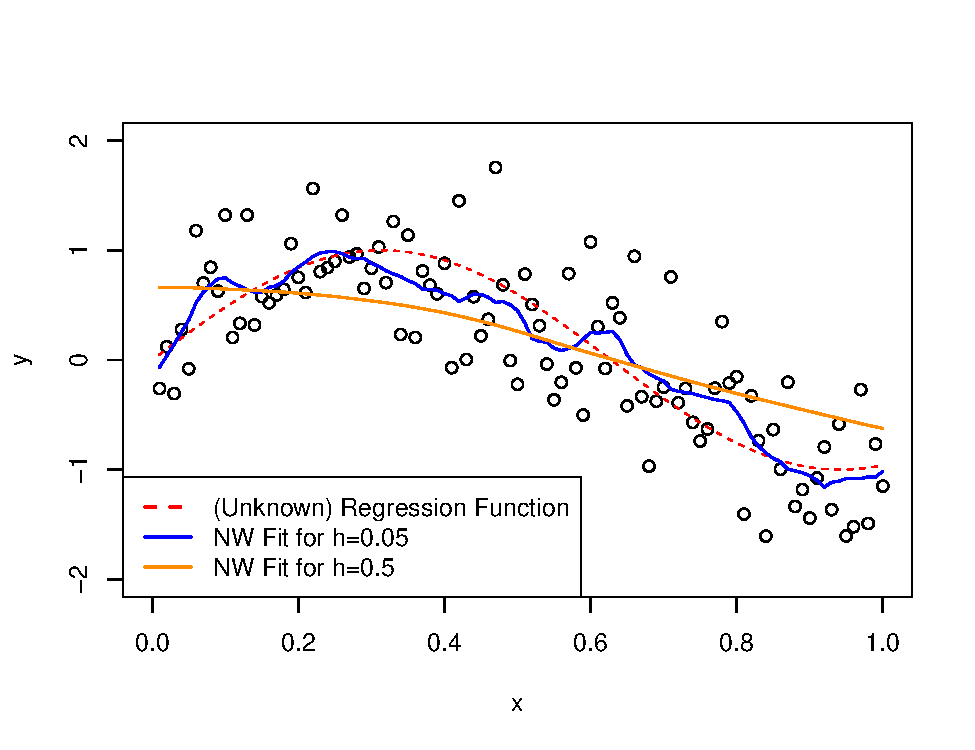
\includegraphics[width=\maxwidth]{figure/unnamed-chunk-23-1} 

}


\end{knitrout}
 




% \end{slide*}
% \begin{slide*}
%  Kernel estimator (Gaussian kernel, $h=1$)
% \begin{center}
% \epsfig{ file=/Pics/chap1/ageker10.eps, width=10cm,height=6cm}\end{center}
% \bigbreak\noindent Kernel estimator (Gaussian kernel, $h=4$)
% \begin{center}
% \epsfig{ file=/Pics/chap1/ageker40.eps, width=10cm,height=6cm}\end{center}
% \end{slide*}
% \begin{slide*}
%  Kernel estimator (Gaussian kernel, $h=10$)
%  \begin{center}
% \epsfig{ file=/Pics/chap1/ageker100.eps, width=10cm,height=6cm}\end{center}
% \bigbreak\noindent Kernel estimator (Gaussian kernel, $h=25$)
% \begin{center}
% \epsfig{ file=/Pics/chap1/ageker250.eps, width=10cm,height=6cm}\end{center}
% \end{slide*}
% 
% 

\newpage
\textbf{MSE and Optimal Bandwidth for Equidistant Design} 
\bigbreak\noindent
Assumptions: 
\begin{itemize}
\item Equidistant  Design on $[a,b]=[0,1]$. I.e., with
$X_{i+1}-X_i=1/n$
\item $m$ twice continuously differentiable.
\item Second order kernel with compact
support $[-1,1]$.
\item $n\rightarrow\infty$, $h\rightarrow 0$, $nh\rightarrow\infty$
\end{itemize}

\bigbreak

This is the simplest possible situation. Then for any x in the interior of $[0,1]$
$$\frac{1}{nh} \sum_{j=1}^n K\Big({x-X_j\over h}\Big)\rightarrow 1,$$
and
$$\frac{1}{nh} \sum_{j=1}^n K\Big({x-X_j\over h}\Big)\,m(X_i)=\int_{-1}^1 K\Big({x-u\over h}\Big)\,m(u)du+o\left(\frac{1}{n}\right)$$

Straightforward Taylor expansions then yield

\begin{itemize}
\item Local bias ($x$ in the interior of $[0,1]$): 
$$\tilde m_h(x)=\E_\epsilon\left(\hat m_h(x)\right)
=m(x)+\frac{1}{2} h^2\,m''(x) \nu_2(K)+o(h^2)$$
 $$\Rightarrow (\operatorname{Bias}({\hat m}_ h(x)))^2=(m(x)-\tilde m_h(x))^2= {1\over 4}  h^4 m''(x)^2\nu_2(K)^2
 +o(h^4),$$
where $\nu_2(K)=\int_{-\infty}^\infty K(z)z^2dz$.
\item Local variance ($x$ in the interior of $[0,1]$): 
 $$\V_\epsilon(\hat m_h(x))={\sigma^2\over nh}  R(K) +o(\frac{1}{nh}),$$
where $R(K)=\int_{-\infty}^\infty K(z)^2dz$.
\end{itemize}

\bigskip
The local mean squared error is then given by:
$$\begin{array}{ll}
&\operatorname{MSE}(\hat m_h(x))
= (\operatorname{Bias}_\epsilon({\hat m}_ h(x)))^2
+ \V_\epsilon({\hat m}_ h(x))\\
&= {1\over 4}  h^4  m''(x)^2\nu_2(K)^2 +{\sigma^2\over n
h}  R(K)+o(h^4+\frac{1}{nh})
\end{array}$$


The optimal (local) bandwidth balancing bias and variance:
$$ h_{opt,x}=n^{-1/5}\biggl({R(K) \over
m''(x)^22\nu_2(K)^2}\biggr)^{1/5}$$

This implies $\operatorname{MSE}(\hat m_{h_{opt}}(x))=O(n^{-4/5})$.


\newpage

\textbf{NW-Estimator as a Local Polynomial (degree=0) Regression}
\bigskip

The NW-Estimator can be seen as a \textbf{locally} weighted least squares estimate with only an intercept as regressor. That is, we can simply use 
\begin{center}
\texttt{lm(y $\sim$ 1, weights=w)}
\end{center}
with local weights $\texttt{w}=w(x,X_i,h)$ in order to compute the NW-estimator. But this is then nothing else then performing polynomial regression (with degree zero) that is using only a weighted subset of the total data. I.e., a local polynomal regression (with degree zero).

\bigskip

The following R-Code visualizes this:
\begin{knitrout}
\definecolor{shadecolor}{rgb}{0.878, 0.918, 0.933}\color{fgcolor}\begin{kframe}
\begin{alltt}
\hlcom{# Define the point at which m(x) shall be estimated:}
\hlstd{x0}       \hlkwb{<-} \hlnum{0.2}
\hlcom{# Choose a bandwidth:}
\hlstd{h}        \hlkwb{<-} \hlnum{0.1}
\hlcom{# Compute the local weights:}
\hlstd{w}        \hlkwb{<-} \hlkwd{w_fun}\hlstd{(}\hlkwc{x0} \hlstd{= x0,} \hlkwc{x_vec} \hlstd{= x_vec,} \hlkwc{h} \hlstd{= h)}
\hlcom{# Center the X-data around x:}
\hlstd{db_x0}    \hlkwb{<-} \hlkwd{data.frame}\hlstd{(}\hlstr{"y"}\hlstd{=y_vec,} \hlstr{"x"}\hlstd{=x_vec}\hlopt{-}\hlstd{x0)}
\hlcom{# Computing the Nadaraya-Watson estimate }
\hlcom{# (= Fitting a local constant):}
\hlstd{NW_estim} \hlkwb{<-} \hlkwd{lm}\hlstd{(y} \hlopt{~} \hlnum{1}\hlstd{,} \hlkwc{data}\hlstd{=db_x0,} \hlkwc{weights}\hlstd{=w)}
\hlcom{# Save the NW estimate }
\hlcom{# (=estimate of intercept-parameter)}
\hlstd{y0_NW}    \hlkwb{<-} \hlkwd{coef}\hlstd{(NW_estim)}
\end{alltt}
\end{kframe}
\end{knitrout}
 
R-Code to visualize the NW-Estimator as a \emph{locally} weighted least squares estimator:
\begin{knitrout}
\definecolor{shadecolor}{rgb}{0.878, 0.918, 0.933}\color{fgcolor}\begin{kframe}
\begin{alltt}
\hlcom{# Plot: #################################}
\hlkwd{plot}\hlstd{(db,} \hlkwc{cex}\hlstd{=}\hlkwd{abs}\hlstd{(w)}\hlopt{*}\hlnum{4}\hlstd{,} \hlkwc{type}\hlstd{=}\hlstr{"n"}\hlstd{)}
\hlcom{# light-gray background}
\hlkwd{rect}\hlstd{(}\hlkwd{par}\hlstd{(}\hlstr{"usr"}\hlstd{)[}\hlnum{1}\hlstd{],} \hlkwd{par}\hlstd{(}\hlstr{"usr"}\hlstd{)[}\hlnum{3}\hlstd{],} \hlkwd{par}\hlstd{(}\hlstr{"usr"}\hlstd{)[}\hlnum{2}\hlstd{],}
     \hlkwd{par}\hlstd{(}\hlstr{"usr"}\hlstd{)[}\hlnum{4}\hlstd{],} \hlkwc{col} \hlstd{=} \hlkwd{gray}\hlstd{(}\hlnum{.80}\hlstd{),} \hlkwc{border}\hlstd{=}\hlkwd{gray}\hlstd{(}\hlnum{.80}\hlstd{))}
\hlcom{# plotting All data pairs (Y_i, X_i)}
\hlkwd{points}\hlstd{(db,} \hlkwc{pch}\hlstd{=}\hlnum{21}\hlstd{,} \hlkwc{cex}\hlstd{=}\hlnum{.3}\hlstd{,} \hlkwc{bg}\hlstd{=}\hlkwd{gray}\hlstd{(}\hlnum{.5}\hlstd{),}
       \hlkwc{col}\hlstd{=}\hlkwd{gray}\hlstd{(}\hlnum{.5}\hlstd{),} \hlkwc{lwd}\hlstd{=}\hlnum{1}\hlstd{)}
\hlcom{# dark-gray background for the interval [x0-h, x0+h]}
\hlkwd{rect}\hlstd{(x0}\hlopt{-}\hlstd{h,} \hlkwd{par}\hlstd{(}\hlstr{"usr"}\hlstd{)[}\hlnum{3}\hlstd{], x0}\hlopt{+}\hlstd{h,} \hlkwd{par}\hlstd{(}\hlstr{"usr"}\hlstd{)[}\hlnum{4}\hlstd{],}
     \hlkwc{col} \hlstd{=} \hlkwd{gray}\hlstd{(}\hlnum{.70}\hlstd{),} \hlkwc{border}\hlstd{=}\hlkwd{gray}\hlstd{(}\hlnum{.70}\hlstd{))}
\hlcom{# re-draw the outer box of the plot}
\hlkwd{box}\hlstd{()}
\hlcom{# plotting the data pairs (Y_i, X_i), }
\hlcom{# plus visualization of the weigths}
\hlkwd{points}\hlstd{(db,} \hlkwc{pch}\hlstd{=}\hlnum{21}\hlstd{,} \hlkwc{cex}\hlstd{=}\hlkwd{abs}\hlstd{(w)}\hlopt{*}\hlnum{1.8}\hlstd{,} \hlkwc{bg}\hlstd{=}\hlkwd{gray}\hlstd{(}\hlnum{0}\hlstd{),}
       \hlkwc{col}\hlstd{=}\hlkwd{gray}\hlstd{(}\hlnum{0}\hlstd{),} \hlkwc{lwd}\hlstd{=}\hlnum{1}\hlstd{)}
\hlcom{# Estimated local constant regression line:}
\hlkwd{lines}\hlstd{(}\hlkwc{x}\hlstd{=}\hlkwd{c}\hlstd{(x0}\hlopt{-}\hlstd{h, x0}\hlopt{+}\hlstd{h),} \hlkwc{y}\hlstd{=}\hlkwd{c}\hlstd{(y0_NW,y0_NW),} \hlkwc{col}\hlstd{=}\hlstr{"red"}\hlstd{)}
\hlcom{# True regression function m(x):}
\hlkwd{lines}\hlstd{(}\hlkwc{x}\hlstd{=x_vec,} \hlkwc{y}\hlstd{=}\hlkwd{sin}\hlstd{(x_vec} \hlopt{*} \hlnum{5}\hlstd{),} \hlkwc{col}\hlstd{=}\hlstr{"red"}\hlstd{,} \hlkwc{lty}\hlstd{=}\hlnum{2}\hlstd{)}
\hlcom{# Estimated point: \textbackslash{}hat\{m\}_h(x0)}
\hlkwd{points}\hlstd{(}\hlkwc{y} \hlstd{= y0_NW,} \hlkwc{x} \hlstd{= x0,} \hlkwc{pch}\hlstd{=}\hlnum{21}\hlstd{,} \hlkwc{bg}\hlstd{=}\hlstr{"red"}\hlstd{,} \hlkwc{col} \hlstd{=}\hlstr{"red"}\hlstd{)}
\hlkwd{abline}\hlstd{(}\hlkwc{v}\hlstd{=x0,} \hlkwc{lty}\hlstd{=}\hlnum{2}\hlstd{,} \hlkwc{lwd}\hlstd{=}\hlnum{.8}\hlstd{)}
\end{alltt}
\end{kframe}

{\centering 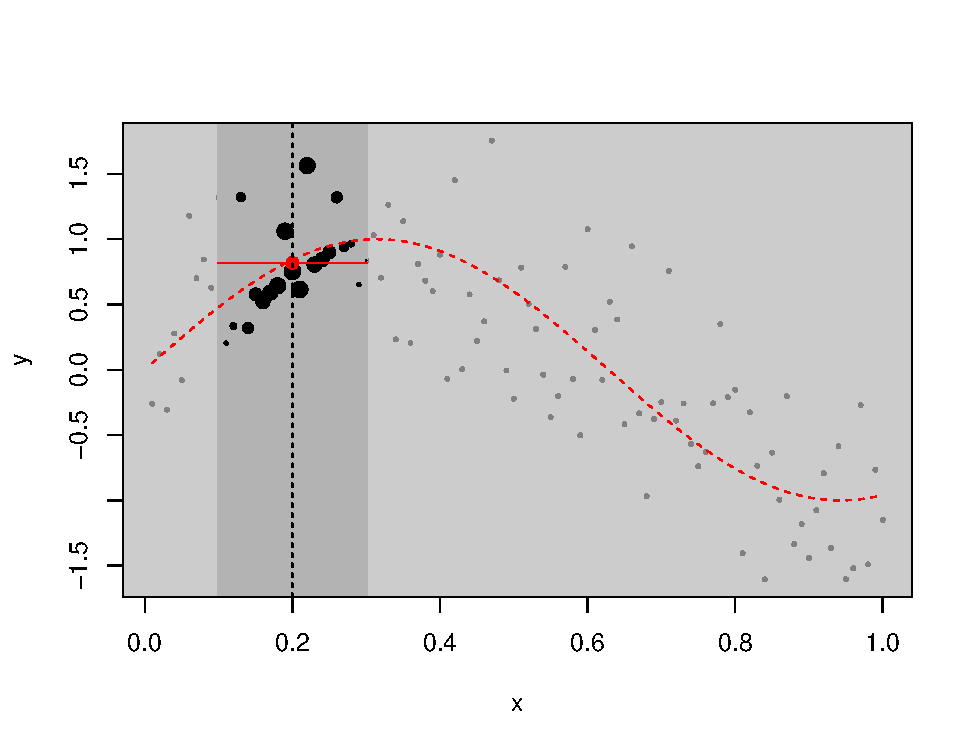
\includegraphics[width=\maxwidth]{figure/unnamed-chunk-25-1} 

}


\end{knitrout}


% %\item
% %Ein optimale {\it globale} Bandbreite  $ h_{opt}$
% %bestimmt sich durch Mitteln ?ber die verschiedenen lokal optimalen $ h_{opt,x}$
% %\item F?r die das GCV Kriterium minimierende Bandbreite $ h_{GCV}$ gilt
% %unter einigen zus?tzlichen technischen Bedingungen, dass ${
% %h_{opt}- h_{GCV}\over h_{opt}}\rightarrow_P 0$ f?r
% %$n\rightarrow\infty$.
% \end{itemize}
% \bigbreak
% 
% %\end{slide*}
% 
% %\begin{slide*}
% \vskip 1cm
% \centerline{\bf Estimation error for random design}
% \bigbreak
% Assumptions: Random design; $X_1,\dots,X_n$ i.i.d. random variables with density $f$ ($f$ is usually
% called ''design density'');\\
%  $m$ twice continuously differentiable; $x$ in the interior of $[a,b]$
% 
% Asymptotic approximations ($n\rightarrow\infty$, $h\rightarrow 0$, $nh\rightarrow\infty$):
% $$Bias_\epsilon^2({\hat m}_ h(x))=\frac{h^4}{4} \nu_2(K)^2 \left( m''(x)+\frac{2m'(x)f'(x)}{f(x)}\right)^2
% +O_P(\sqrt{\frac{h}{n}})o_P(h^2)$$
% and
% $$Var_\epsilon({\hat m}_ h(x))={\sigma^2\over f(x) n
% h}  R(K)+o(\frac{1}{nh}),$$
% %where $\nu_2(K)=\int_{-\infty}^\infty K(z)z^2dz$, $R(K)=\int_{-\infty}^\infty K(z)^2dz$.
% wich implies
% 
% {\small
% $$ MSE({\hat m}_ h(x))=\frac{h^4}{4} \nu_2(K)^2 \left( m''(x)+\frac{2m'(x)f'(x)}{f(x)}\right)^2
% +{\sigma^2 R(K)\over f(x) n
% h}+o_P(h^4+\frac{1}{nh}) $$}
% An optimal local density  $h_{opt,x}$ thus additionally  depends on the values
%  $f(x)$ and $f'(x)$ of the design density at the point $x$.
% \bigbreak
% 
% {\bf Boundary problems:}
%  The accuracy of kernel estimators decreases if the point $x$ of interest is close to one of the
% boundaries $a$ or $b$ of the estimation interval
%  $[a,b]$. If $x=a$ or $x=b$ then
% $Bias^2({\hat m}_ h(x))=O_P(h^2)$ (instead of $Bias^2({\hat m}_ h(x))=O_P(h^4)$ for $x$ in the interior of $[a,b]$). Boundary effects will even dominate the MASE when averaging over all observations. In kernel
% estimation it is thus common practice to exclude all observations in the intervals
% $[a,a+h]$ and $[b-h,b]$ when determining error measures or when computing optimal bandwidths.\\
% Note: Boundary
% effects may be (partially) compensated by suitable modifications of the estimation procedure at boundary points.
% \vskip 1cm
% 
%  {\bf Remark }: In practice the value of $h$ has to depend on the scale of the $X$-variable
% \par\noindent
% $\{X_i\}, h$ $\quad\Leftrightarrow\quad$ $\{10X_i\},10 h$.
% \par\noindent
% Sometimes so-called ''standardized'' bandwidths $c$ are used
% $$ h=cQn^{-1/5}$$
% \begin{itemize}
% \item $Q$: interquartile range of the $X$-Variable
% \item $c\in[0,1]$
% \end{itemize}
% %\end{slide*}
% 
% %\begin{slide*}
% \bigbreak\noindent
% 
%  {\bf Theory of optimal kernels}:
%  \begin{itemize}
%  \item Asymptotically (MSE based on an optimal bandwidth) the
%  Epanechnikov kernel is the optimal kernel function  in the class of all
%  symmetric densities.
%  \par\noindent
%  (criterion: minimal  MSE when using an optimal bandwidth).
% \item However, the Gaussian and biweight kernels are only very slightly less efficient.
% \item Literature: M\"uller, H.G. (1988). {\sl Nonparametric regression analysis
% of longitudinal data}, Springer Verlag, Berlin
% \end{itemize}
% \end{slide*}




















%%%%%%%%%%%%%%%%%%%%%%%%%%%%%%%%%%%%%%%%%%%




%' \textbf{Regression model (general version):}
%' $$
%' Y_i=m(X_i)+\epsilon_i,\quad i=1,\dots,n,
%' $$
%' where:
%' 
%' \begin{itemize}
%' \item $Y_{i}$ response (or dependent) variable
%' \item  $X_{i}\in [a,b]\subset \mathbb{R}$ explanatory variable 
%' \item  The sample (simples setup):  $(Y_i,X_i)$ are i.i.d.
%' \item  Error term (simplest setup): $\epsilon_i$ is i.i.d.~with 
%' \begin{itemize}
%' \item[] $\mathbb{E}(\epsilon_i|X)=\mathbb{E}(\epsilon_i)=0$
%' \item[] $\mathbb{V}(\epsilon_i|X)=\mathbb{V}(\epsilon_i)=\sigma_\epsilon^2$
%' \end{itemize}
%' \end{itemize}
%' 
%' Under this simple setup, we can identify the regression function $m(.)$ by the conditional mean of $Y_i$ given $X_i$:
%' \begin{align*}
%' \E(Y_i|X_i)
%' &=\E(m(X_i)+\epsilon_i|X_i)\\
%' &=\E(m(X_i))+\E(\epsilon_i|X_i)\\
%' &=m(X_i)
%' \end{align*}
%' 
%' 
%' The error term $\epsilon_i$ quantifies the non-systematic (purely random) variances of  $Y_i$ around the regression function $m(x_i)$. Such non-systematic variances can be induced by measurement errors, but also by additional unobserved variables, which have an influence on $Y_i$, however, not on  $X_i$.\\
%' 
%' \textbf{Model Assumption on $m(.)$:}
%' \begin{itemize}
%' \item[]In \textbf{parametric statistics} we additionally need to assume a specific functional form of the regression function $m(.)$. For instance, we would assume that $m(x)=\alpha+\beta x$.
%' 
%' \item[]In \textbf{nonparametric statistics} we would impose only a qualitative assumption on $m(.)$. Typically, it is assumed that the unknown regression function has $2$ or more continuous derivatives. I.e., that $m(.)$ is a sufficiently smooth function.
%' \end{itemize}
%' 
%' \newpage
%' \textbf{Explanatory Variable $X$:}\\[1ex]
%' In regression analysis it is often important how the regressors $X_1,\dots,X_n$ have been generated. We differentiate between a \textbf{fixed} and a \textbf{random} design:
%' 
%' \begin{description} 
%' \item[\textbf{Fixed Design:}] The observations $X_1,\dots,X_n$ are fixed (i.e., non-stochastic) values. 
%' Example: crop yield $Y$ in dependency of fixed amounts of fertilizer $X$. \\
%' Important special case: \textbf{equidistant design}, where all points have equal distances, i.e., $X_{i+1}-X_i=\frac{b-a}{n}$.
%' 
%' \item[\textbf{Random Design:}] The observations $X_1,\dots,X_n$ are realizations of an i.i.d.~random sample with density $f_X$, where $X_i$ is uncorrelated with the error term  $\epsilon_i$. \\
%' We denote the density function $f_X$ as the \textbf{design-density}.
%' \end{description}
%' 
%' This is how you can simulate artifical data for a univariate nonparametric regression model:
%' <<fig.width=6, fig.height=5>>=
%' # Generate some data: ######################
%' n      <- 100     # Sample size
%' # Explanatory variable X
%' # x_vec  <- (1:n)/n # Equidistant X 
%' x_vec  <- sort(runif(n)) # Random design 
%' # Gaussian iid error term: 
%' e_vec  <- rnorm(n = n, mean = 0, sd = .5)
%' # Repsonse variable Y
%' y_vec  <-  sin(x_vec * 5) + e_vec
%' # Save all in a dataframe
%' db     <-  data.frame(x=x_vec,y=y_vec)
%' ############################################
%' ## Plot:
%' plot(db, ylim=c(min(y_vec),max(y_vec)+1), xlim=c(0,1))
%' # Add the true regression function m(x):
%' lines(x=x_vec, y=sin(x_vec * 5), col="red", lty=2, lwd=2)
%' # Add a legend:
%' legend("topright", 
%'  c("(Unknown) Regression Function m", 
%'    expression(paste("Sample Points: (",Y[i],X[i],")"))), 
%'  col=c("red","black"), pch=c(NA,1), lty=c(2,NA), 
%'  lwd=c(2, 0), pt.lwd=c(0,1))
%' @
%' 
%' 
%' % # Epanechnikov kernel function
%' % epanech_kern_f   <- function(u){ifelse(abs(u)<=1, ( 3/ 4) * (1-u^2), 0)}
%' % 
%' % # Function to compute Epanechnikov kernel-weights:
%' % w_fun <- function(x0, x_vec, h){
%' %   u     <- (x_vec - x0)/h
%' %   epa_w <- epanech_kern_f(u=u)
%' %   return(epa_w)
%' % }
%' % 
%' % # Choose a bandwidth:
%' % h   <- 1
%' % 
%' % # Computing the corresponding weights (Take a look at the weights!)
%' % w_fun(x0 = x_vec[1], x_vec = x_vec, h = h) 
%' % 
%' % # Computing the Smoothing-Matrix S_h:
%' % S_h_mat <- matrix(NA, nrow = n, ncol = n)
%' % for(i in 1:n){
%' %     S_h_mat[i,] <- w_fun(x0 = x_vec[i], x_vec = x_vec, h = h) / 
%' %                       sum(w_fun(x0 = x_vec[i], x_vec = x_vec, h = h) )
%' % }
%' % round(S_h_mat[1:10, 1:10], digits=5)
%' % 
%' % # Compute the estimates: \hat{m}_h(X_1),...,\hat{m}_h(X_n)
%' % m_hat <- S_h_mat %*% y_vec
%' % 
%' % ## Plot ####################################################
%' % # Data points:
%' % plot(db, ylim=c(-2,2), xlim=c(0,1))
%' % # Plotting the fitted values \hat{m}_h(X_1),...,\hat{m}_h(X_n)
%' % lines(y = m_hat, x = x_vec, col="red", lwd=2)
%' % # Add the true regression function m(x):
%' % lines(x=x_vec, y=sin(x_vec * 5), col="red", lty=2, lwd=2)
%' 
%' 
%' 
%' 
%' \subsection{The Nadaraya Watson Estimator}



























% \bibliography{bib/lib.bib}
% \bibliographystyle{plainnat}
\end{document}
